%% File Name : PhysNote_QM.tex
%% 説明      : 量子力学
%%
%%**************************************************************************************************
%===================================================================================================
%  Chapter : 原子論
%  説明    : 量子力学に入る前に,前置きとして,原子という考え方の妥当性を考える
%===================================================================================================
\chapter{原子論}
%   %-----------------------------------------------------------------------------------------------
%   %  Input
%   %    File Name : PhysNote_QM_Particles.tex
%   %    説明      : 原子論に至るまでのの記述(化学の歴史)
%   %-----------------------------------------------------------------------------------------------
        %   %==========================================================================
%   %  Section
%   %==========================================================================
    \section{原子,分子の概念の導入}
        \begin{mycomment}
            最初に「化学」の分野で習う法則を確認するが,あくまでも量子力学を確認するためである.多
            くの量子力学の教科書は,「物質は多数の原理や分子の運動である」ということが当然のように記述
            されている.しかし,原子を肉眼で確認することは不可能である.どのように「物体は多数の原子や
            分子の集合である」ことを見出したのかについては書かれていないことが多い.

            実は,分子や原子の概念は「化学」の分野で最初に導入された.当然,分子・原子を観測することは
            できなかったのだが,化学反応という現象を説明するには,原子や分子という概念を導入する必要が
            あったのである.そこで,このノートでは分子や原子の導入のために,簡単な化学反応を最初に確
            認したいのである.

            なぜ,物質は小さな原子の集まりである,といわれるのだろうか.
            ここでは,その原子という概念の導入となる,
            いくつかの化学の法則を見ていくことにしよう.

            使用する教科書は,
                \begin{itemize}
                    \item 竹内 敬人 [著],
                            『化学の基本6法則』,岩波ジュニア新書,1982
                    \item 小川 岩雄 [著],
                            『原子と原子核』,共立出版,2008
                    \item Steven Weinberg [著],本間 三郎 [訳],
                            『(新版)電子と原子核の発見』,ちくま学芸文庫,2009
                    \item Isaac Asimov [著],玉虫 文一$\cdot$竹内 敬人 [訳]
                            『化学の歴史』,ちくま学術文庫,2010
                \end{itemize}
            である.
        \end{mycomment}

%       %======================================================================
%       %  Subsection
%       %======================================================================
        \subsection{定比例の法則}
            リヒター
                \footnote{
                    Jeremias Benjamin Richter (1762--1807,ドイツ),化学者
                },
            プルースト
                \footnote{
                    Joseph Louis Proust (1754--1826,フランス),化学者
                }
            は定比例の法則を発見する.

                \begin{myshadebox}{定比例の法則}
                    与えられた物質の成分元素の質量比は一定である.
                \end{myshadebox}

            水を例にとってこの法則を考えてみる
                \footnote{
                    気体の例を挙げるよりも,身近な水の例を挙げたほうがわかりやすいと思う.
                }.
            水は水素と酸素から構成されている.定比例の法則が意味するのは,水を構成する水素と酸
            素の質量比が一定だということである.もっと簡単にいえば,「水を構成する水素と酸素は
            いつでも同じ割合いなっている」ということである.具体的には,水を構成する水素と酸素
            の比は,水素:酸素 $=$ 1:8 である
                \footnote{
                    ここで注意すべきなのは,“水素が1つに対して酸素が8つということではない”
                     ということである.あくまでも質量比である.水素1[$\mathrm{g}$] に対して,
                     8[$\mathrm{g}$] の酸素が反応するということである.9[$\mathrm{g}$]の酸素が
                     存在しても,そこに水素が1[$\mathrm{g}$]しかない場合,この水素と酸素が反応
                     した後,1[$\mathrm{g}$]の酸素が残るのである.
                }.

%       %======================================================================
%       %  Subsection
%       %======================================================================
        \subsection{倍数比例の法則}
            ドルトン
                \footnote{
                    John Dalton(1766--1844,イギリス):原子説を強く唱えた科学者.ボイルやラヴォアジエ
                    らの実験事実に基づく理論構築を行った.
                }
            はこの \textbf{倍数比例の法則} を提唱し,物質の原子説を発表した.この理論により,原子説が有力になり,
            物質の変化を原子の観点から,考察されるようになった.
                \begin{myshadebox}{倍数比例の法則}
                    2種類の元素が2つ以上の化合物を形成するとき,一方の元素の一定量と化合する他方の
                    質量は互いに簡単な整数比になる.
                \end{myshadebox}

            同じ二つの種類の元素からなる化合物を,2種類考えてみよう.例えば,CO(一酸化炭素)と
            CO${}_{2}$にしよう.たしかに,COとCO${}_{2}$は,両方ともにC(炭素)とO(酸素)の二種類の元
            素から構成されている.
            例えば,炭素Cを一定量とすると,一酸化炭素と二酸化炭素のそれぞれに含まれる酸素の比は 1:2 である
                \footnote{
                    現在の化学記号は,すでに倍数比例の法則が反映されているため,
                    この法則を説明するのに化学記号を使って説明を行うと,
                    記号を見れば明らかではないか,と思われるかもしれない.
                }.

%       %======================================================================
%       %  Subsection
%       %======================================================================
        \subsection{ドルトンの原子説}
            物質を構成するものには基本的なものがある.この基本的の物質を“\textbf{元素}(element)”
            という.もう少し正確に元素を定義するならば,
                \begin{center}
                    “\textbf{元素}”とは「それ以上に単純な物質に分けられないもの」である.
                \end{center}
            と言える.「元素」に“ ”をつけたのは,現在は元素の定義として,この定義を用
            いていないからである.現在は,上の「それ以上に単純な物質に分けられないもの」で定義され
            る量は,\textbf{単体} とよばれている.

            ドルトンから始まる原子説は,単に化学現象を理論的に説明するために作られた,
            思考上の概念であった.原子の実在性は,この後,物理学者に再度疑われ
                \footnote{
                    力学史で有名なマッハは,原子説に対して批判的であったらしい.
                },
            さらなる実験がなされることになる.

%       %======================================================================
%       %  Subsection
%       %======================================================================
        \subsection{気体反応の法則,アヴォガドロの分子説}
            ゲイ・リュサック
                \footnote{
                    Joseph Louis Gay-Lussac(1778--1850, フランス):フランスの
                    化学者.
                }
            は,気体同士の反応に関する法則を発見した.
            \begin{myshadebox}{気体反応の法則}
                気体間が化学反応するとき,反応する気体の体積と生成する気体の体積の間には簡単な
                整数比が成立する.
            \end{myshadebox}

%   %==========================================================================
%   %  Section
%   %==========================================================================
    \section{原子模型}
            \begin{mycomment}
                \textbf{原子模型} とは 原子構造の模型のことをいう.
                化学の世界で,原子の存在が確かになってくると,その次の段階として,原子の構造に興味
                が湧くのは当然のことだろう.ここでは,原子の構造はどのようになっているかを考えた人
                の,いくつかの提案(構造の模型)を見ていくことにしよう.はじめに注意しておくと,これ
                らの模型は量子力学的に間違ったものである.しかし,量子力学を考慮しない範囲では有用
                な考え方であり,実際に物体をマクロで考えるときにはこの原子模型を用いて話をされるこ
                とが多い.
            \end{mycomment}

%       %======================================================================
%       %  Subsection
%       %======================================================================
        \subsection{電子の発見}
            電子の発見は,マクスウェルによって電磁気学が確立された後のことである.電磁気学の部分で保留
            にしていた電子の発見について,ここで確認しておこう.原子は電気的に中性である.「電気的
            に中性」というのは正の電荷も負の電荷ももたないということである.原子がその内部に電子を
            含むので,この電子のもつ負の電荷とちょうど相殺するような正電荷を原子はもっていることに
            なる
                \footnote{
                    「物質を構成する最小の単位は原子である」という仮定をしていることを前提とした主
                    張である.
                }.
            この正電荷が陽子である.原子がどのような形で陽子をもっているかについては,2通り考えら
            れる.1つは陽子と電子が混在しているものである.この構造はトムソンによって提案されたの
            で \textbf{トムソンの原子模型} とよばれる.もう一つは,陽子の周りを電子が回転していると
            いうものである.この構造は,日本人の長岡半太郎によって提唱されたものである.この長岡の
            原子模型では,電子は平面上の楕円軌道を描くとされる.土星のような模型である.土星の輪が
            電子の描く軌道に相当する.この模型の拡張とのいうべきものが,ラザフォード
                \footnote{
                    Ernest Rutherford(1871--1937, イギリス):原子核の発見(実験),$\alpha$線と
                    $\beta$線の発見などで有名.放射線に $\gamma$線という名前を与えたのもこの人.
                    元素崩壊と放射線の業績(化学)を理由に,ノーベル化学賞を受賞している.
                }
            によって提案され
            た.\textbf{ラザフォードの原子模型} では,電子は1つの平面における単なる楕円軌道ではなく
            ,楕円軌道が刻々と変化するというものである.ラザフォードらの実験によれば,
            原子の形はラザフォード模型であることが確認される.しかし,この原子模型には欠
            点がある.後で確認することだが,陽子の周りを電子が回転すると電磁波が生じる.この電磁波
            は電子のもつエネルギーを外部に放射してしまう.このため,原子の速度が減少し,電子が陽子
            の周りを回転するために必要な速度が保てなくなる.すなわち,電子が陽子とくっついて,原子
            がつぶれてしまうのである.このラザフォード模型の欠点は,\textbf{量子力学} という新しい物
            理学の分野を待たなければ解決することができない.

            話が前後するが,電子のもつ電気量の測定は「ミリカンの油滴実験」が有名である.もちろん,
            この実験の原理はマクスウェル方程式によって説明される.

%       %==========================================================================================
%       %  SubSection
%       %==========================================================================================
        \subsection{ラザフォードの原子模型(原子核の発見)}
            原子構造は,正電荷を持った原子核の周りに,負電荷を持った電子が周っている模型が
            知られている.こうした今日知られている原子模型は,ラザフォードによるものである.
            ラザフォードは,原子構造を模索している中の実験で,奇妙な結果(\textbf{ラザフォード散乱})を得て,
            この結果から,現在知られている原子模型作り上げた.

            ラザフォードは,金属の薄膜に$\alpha$線を照射して,その透過具合や散乱の程度を調べる
            実験を行った.その結果は,ある割合で,$\alpha$線が透過せずに跳ね返ってくること
            が判明した.
                \begin{figure}[hbt]
                    \begin{center}
                        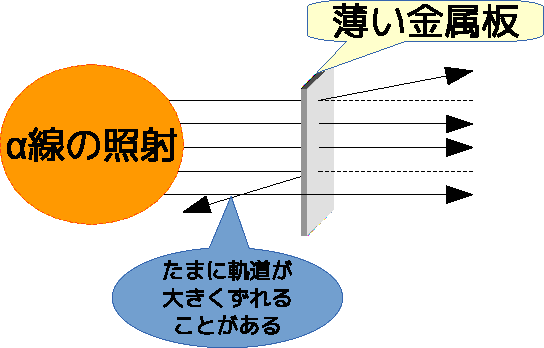
\includegraphics[keepaspectratio, width=4.6cm,height=2.95cm,clip]{RutherfordScattring.pdf}
                        \caption{ラザフォード散乱}
                        \label{fig:RutherfordScattring}
                    \end{center}
                \end{figure}

            その結果から,原子の構造は中心に正電荷をもった粒子があり,
            その正電荷の周囲に電子が存在する,という構造を導き出した
                \footnote{
                    (参考)新版 電子と原子核の発見,S.ワインバーグ [著],本間三郎 [訳],ちくま文芸文庫:
                     特に,第4章に原子核に関する実験について詳しく書かれている.
                     この本には,トムソンの陰極線に関する実験や,ミリカンの電子に関する実験なども丁寧に
                     書かれている.
                }.
            電磁気学とニュートン力学に基づいて発案されたこの原子模型は,現在の量子力学では
            否定されてしまう.しかし,化学を考える場合や電子回路と考える場合などは,このモデルで
            十分であることが多い.
                \begin{figure}[hbt]
                    \begin{center}
                        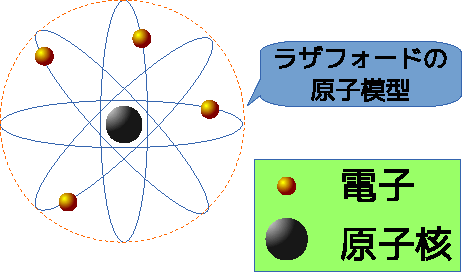
\includegraphics[keepaspectratio, width=4.0cm,height=2.56cm,clip]{RutherfordAtomModel.pdf}
                        \caption{ラザフォードの原子模型}
                        \label{fig:RutherfordAtomModel}
                    \end{center}
                \end{figure}

        \begin{memo}{トムソンの原子模型}
            ラザフォードによる原子構造の発見よりも前に,トムソンは \textbf{陰極線} という
            現象を発見している.陰極線とは,真空中に2つの電極を用意し,この電極間に高電圧をかけると,
            負電極から正電極に向かって何らかの粒子が飛ぶ現象である.陰極線という名前は,
            その性質からトムソン自身によって与えられた.実は,この陰極線は後に電子であることが判明する.

            電子は,負極から正極へと走ることから,負電荷であることがわかる.多くの物質は電気的に
            中性であることから,電子の負電荷はどこかで中和されているはずである.要するに,どこかに
            正電荷をもつ部分があるということだ.

            トムソンの時代には,物質は原子から構成されているという
            ことは,仮説でしかなかったが,トムソンはこの仮説を支持していた.そこで,トムソンは
            原子の模型として,正電荷をもつ領域内に電子がその正電荷を中和するように存在するという,
            原子模型を提唱した.この原子模型を \textbf{トムソンの原子模型} という.
                \begin{figure}[hbt]
                    \begin{center}
                        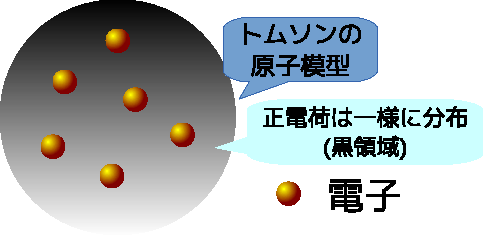
\includegraphics[keepaspectratio, width=5.05cm,height=2.5cm,clip]{TomsonAtomModel.pdf}
                        \caption{トムソンの原子模型}
                        \label{fig:TomsonAtomModel}
                    \end{center}
                \end{figure}
        \end{memo}

        \begin{memo}{長岡の原子模型}
            日本の物理学者に,長岡半太郎
                \footnote{
                    長岡半太郎(1865--1950, 日本):東京大学出身の,日本の物理学の先駆者的存在.土星型の
                    原子模型を提唱したことで有名.後世の教育にも努力された.
                }
            という人物がいる.長岡も原子模型を
            提唱していたらしく,Webサイトを検索するといくつかヒットする.
            電気学会の電磁気学の教科書にも紹介されている.長岡が提唱した
            原子模型は,ラザフォードの原子模型のを2次元にしたようなもので,
            よく化学の教科書に描かれているような元素の図がそのイメージに一致する.
                \begin{figure}[hbt]
                    \begin{center}
                        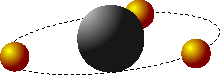
\includegraphics[keepaspectratio, width=3.8cm,height=1.3cm,clip]{NagaokaAtomModel.pdf}
                        \caption{長岡の原子模型}
                        \label{fig:NagaokaAtomModel}
                    \end{center}
                \end{figure}
        \end{memo}


        \begin{memo}{原子は本当に存在するのか}
            「原子」という概念は化学,つまり,物質の性質やその反応を理解するために導入されたもので
            ある.この「原子」という概念を導入することで,が矛盾なくしかも説明がスマートに行えるよ
            うになった.「原子」という概念を導入すれば,確かに,理論を綺麗に組み立てられることは確
            かであるが,実際に,「原子」そのものを見て,その存在を確認したわけではない.では,「原
            子」は,あくまでも理論を組み立てる上で導入する,“仮想”のもので,実際には存在しないも
            のなのだろうか.確かに,肉眼で
                \footnote{
                    あるいは,顕微鏡などで拡大して.
                }
            確認するまで,その存在を認めないと考えるならば,「原子」はただの仮想のものにすぎない.
            そうなると,現実には「原子」は存在せず,何かそれに変わるようなものがあると考えて,それ
            は今の人間には「原子」としてしか認識できないと考えることになるだろう.確かにそうかもし
            れない.この考えを完全に否定することはできない.

            しかし,科学を考える上で,このような考えは余り好ましくないと思う.科学の理論を支え
            る基板---つまり法則は,あくまでも“仮説”である.となれば,「原子」の存在を疑うことは
            ,法則を疑うことにつながる.科学は実験で得た結果に基づいて,推論し理論を組み立てていく
            作業である.それが,絶対に現実の世界と一致している必要はないのである.例えば,ニュートン力
            学は,アインシュタインによって,修正を加えられている.それまで,ニュートン力学はどのよう
            な場合でも
            成立すると考えられてきたと思うが,現実は違っていた
                \footnote{
                    ニュートン力学が仮定から完全に間違っていたわけではなかった.アインシュタインは,
                    考察対象と
                    なる系の速度が光速 $c$ に比べて,とても遅いことを暗黙の内に仮定していることを
                    指摘しただけである.そして,その修正とは,光速 $c$ に近い速度で運動する系でも
                    ,理論が矛盾なく成立するように拡張したものである.理論が全く書き換えられたわけ
                    ではない.理論には暗黙の内に仮定しているものがあるが,その暗黙の仮定は理論成立
                    時には気付けない.しかし,後に科学が発展して,“暗黙の内の仮定”に気付いたので
                    あれば,その都度,理論に修正を加えていけばよいのだ.
                }.
            ニュートン力学の修正のきっかけは,思考の範囲が広がったことと,実験の技術が向上したことに伴
            って,新しい実験結果を得ることができたからである.

            科学の理論とは,実験結果から推測される仮定に基づいて,構築されるものである.数学との違
            いをはっきりと意識させられるところである.

            このようなことから,原子の存在を,肉眼で観測できないからといって,疑う事は避けないとい
            けない.「原子」の存在を仮定して,現象の説明がスマートにできるのであれば,科学的に,“
            そこには「原子」がある”と主張されるのである.そしてこのとき,「原子」は科学的に実在す
            るのである.理論と実験結果の矛盾を見つけるまでは,「原子」の存在を仮定して話を進めてい
            くべきだ.
        \end{memo}


%           %==================================================================
%           %  Subsubsection
%           %========================s==========================================
%            \subsubsection{}

%   %==========================================================================
%   %  Section
%   %==========================================================================
    \section{原子核の構造}
%       %==========================================================================================
%       %  SubSection
%       %==========================================================================================
        \subsection{ウランの発見}
            クラプロート
                \footnote{
                    Martin Heinrich Klaproth(1743--1817, ドイツ):
                    化学者,薬剤師として活躍.
                    ウラン(酸化ウラン)の発見者として有名.
                }
            により,ウラン
                \footnote{
                    Uran,もしくは,Uranium
                }
            を発見する.

            クラプロートは,薬剤師としてドイツ各地で活躍していたが,
            薬学による治療では満足できず,化学的な手段に手を広げようとし,
            銀の発掘現場にて新たな鉱物が発見されたという情報聞をきつけ,
            閃ウラン鉱より,酸化ウランを取り出し発見した.
            「ウラン」の命名由来は,1781年にイギリスの天文学者ハーシェル
                \footnote{
                    Sir Frederick William Herschel(1738--1822, イギリス):
                    ドイツ生まれ.イギリスにわたり,音楽家として活躍する.
                    天文学にも興味を持ち,自身の手により望遠鏡を作成している.
                    その後,天王星を発見し,天文学の研究に専念する.

                    ドイツ語名ではFriedrich Wilhelm Herschelであったが,
                    イギリスに渡った後(1757年),Frederick William Herschelと名乗るように
                    なった.
                }
            が新しい惑星を発見し,「Uranus(ウーラノス,天王星)」を名づけたことを受け,
            これを讃えたことによる.

%       %==========================================================================================
%       %  SubSection
%       %==========================================================================================
        \subsection{X線の発見}
            レントゲン
                \footnote{
                    Wilhelm Conrad R\"{o}ntgen(1845--1923, ドイツ):
                    1901年に,第1回ノーベル物理学賞を受賞.受賞理由は
                    ,もちろん,X線の発見(1895年)による.1888年に,
                    マクスウェルが提唱した変位電流の存在を,
                    実験的に確かめている.
                }
            は(偶然的に)X線を発見した.

            放電管(クルックス管
                \footnote{
                    クルックス管:
                    Sir William Crookes(1832--1919, イギリスの物理学者,化学者)
                    による発明品.
                    トムソンの電子発見の説明でよく出てくる,真空管のこと.
                }
            )による放射現象の研究の中,
            感光処理を施した一枚の紙が発光していることに気づき,
            その原因を突き止めた結果,放電管から生じる目に見えない光線が
            放射されているがわかった.この光線が \textbf{X線} と呼ばれるものである
                \footnote{
                    \textbf{レントゲン線} とも呼ばれる.
                }.

%       %==========================================================================================
%       %  SubSection
%       %==========================================================================================
        \subsection{ウランから生じる放射線の発見}
            ベクレル
                \footnote{
                    Antoine Henri Becquerel(1852--1908, フランス):
                    物理学者.1903年に,放射線の発見により,ノーベル物理学賞
                    を受賞している.
                }
            は,ウランによる蛍光作用の研究の中,ウランから目に見えない放射が
            生じていることを発見した.(ポアンカレ
                \footnote{
                    Jules-Henri Poincar\'{e}(1854--1912, フランス):
                    数学者.アインシュタインの特殊相対性理論の先駆けとなる考察
                    (光速不変の原理など)や,ポアンカレ予想などで,その名が有名
                    である.とにかくものすごい数学者.
                }
            による示唆で,ウランの発光作用とX線との関連の研究を促されたらしい.)


%       %==========================================================================================
%       %  SubSection
%       %==========================================================================================
        \subsection{$\alpha$ 線と$\beta$ 線,$\gamma$ 線の発見}
        ラザフォードが $\alpha$ 線と$\beta$ 線を発見する.
        ピエール$\cdot$キュリーが $\gamma$ 線を発見する.


%===================================================================================================
%  Chapter : 量子力学への道のり
%  説明    : 量子という新しい考え方の導入
%===================================================================================================
\chapter{量子力学への道のり}
%   %-----------------------------------------------------------------------------------------------
%   %  Input
%   %    File Name : PhysNote_QM_Intro.tex
%   %    説明      : 量子力学 前史
%   %-----------------------------------------------------------------------------------------------
        %   %==========================================================================
%   %  Section
%   %==========================================================================
    \section{古典物理学の限界}
            \begin{mycomment}
                古典物理学の問題点は,先にあげた原子構造のほかに,固体比熱の問題と黒体輻射の問題が
                ある.固体比熱の問題は「熱・統計物理学」の部分で考えることにして,ここでは,黒体輻射
                    \footnote{
                        「空洞輻射」,「黒体放射」ともよばれる.
                    }
                の問題について考えることにする.
            \end{mycomment}

%       %======================================================================
%       %  Subsection
%       %======================================================================
            \subsection{黒体}
                \textbf{黒体} とはその名の通り,真っ黒な物体である.真っ黒な物体は,色付きの物体と
                違って,全ての電磁波を吸収する
                    \footnote{
                        色つきの物体は一部の色を吸収しその他を反射することで色を出しているのだ.
                    }.
                つまり,どの電磁波も吸収するということで,その意味で偏りのない物体である.また,こ
                ような黒体はそれ自身が熱をもちはじめると,発光し始める.黒体から発光される光は全て
                の波長の電磁波をふくみ,白っぽく光る.もちろん最初は赤い色を発光し,徐々に温度が高
                くなるに連れて光は青色に変化し,最終的に白くなるということである.

                マクスウェルの電磁波理論より,光の色は電磁波の波長 $\nu$ によって決まることがわかる.こ
                の周波数 $\nu$ のときの光の強度を $u(\nu)$ と表現する.
                すると,光の強度 $u(\nu)$ はどのような関数だろうかという疑問が生じるが,古典論から
                光の強度 $u(\nu)$ の具体的な形を導こうとしても,実験と完全に一致する式を導出するこ
                とはなかなかできなかった.以下に実験結果の例を示しておく
                    %\footnote{
                    %    関根 松夫 著,『量子電磁気学』,コロナ社,1996,p7より.
                    %}.

                キルヒホッフ
                    \footnote{
                        Gustav Robert Kirchhoff (1824‐1887,)
                    }
                は

%       %======================================================================
%       %  Subsection
%       %======================================================================
        \subsection{黒体輻射}
            一般に固体は温度を上げていくと赤く光り,さらに温度を上げていくと,しだいに白い光を発す
            るようになる.この現象は \textbf{黒体輻射} とよばれる.
                \begin{figure}[hbt]
                    \begin{center}
                        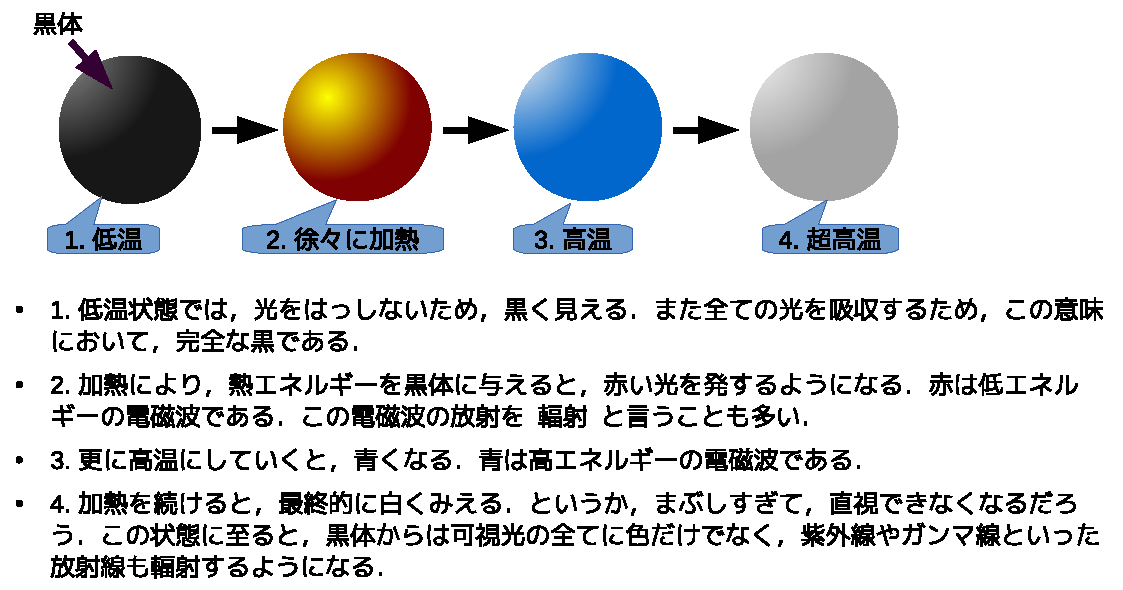
\includegraphics[keepaspectratio, width=7cm,height=5cm,clip]{KokutaiHoushaHakkou1111.pdf}
                        \caption{黒体輻射}
                        \label{fig:kokutai_housha_1}
                        \end{center}
                \end{figure}

            ここで問題とするのは,物体の発する光の色 と そのときの光の強度 の関係で
            ある.実験によれば,図\ref{fig:kokutai_housha_1}のようになる.
                \begin{figure}[hbt]
                    \begin{center}
                        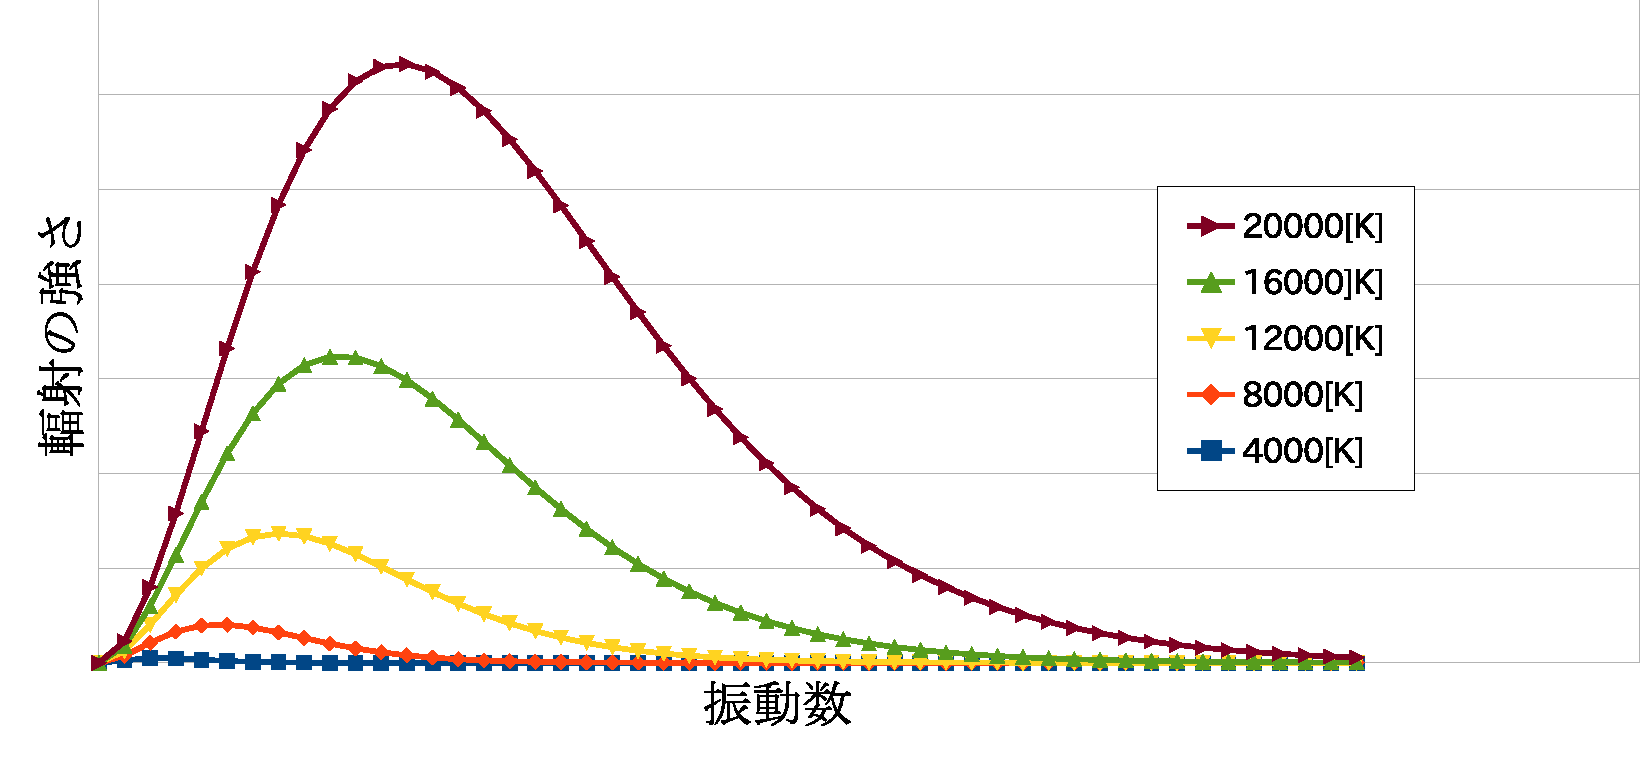
\includegraphics[keepaspectratio, width=7cm,height=4cm,clip]{PlkEq001.pdf}
                        \caption{黒体放射}
                        \label{fig:kokutai_housha_1}
                        \end{center}
                \end{figure}

            縦軸が黒体輻射の強さで,横軸が輻射される電磁波
                \footnote{
                   光とは電磁波のことであった.正確には少し違うが---というのも,可視光以外の電磁波
                   も光と言えると考えれば,電磁波であればそれは光であるとも言える.しか
                   し,光であればそれは電磁波であるとは言い切れない.光子というものが存在するから
                   である.
                }
            の周波数である.このグラフの最大値は,絶対温度によって異なり,温度が高くなるのに伴って最
            大値も上昇する.
            また,最大値となる波長は,温度が高くなるのに伴い,短くなっている.

%       %======================================================================
%       %  Subsection
%       %======================================================================
        \subsection{レイリー$=$ジーンズの公式}
            図\ref{fig:kokutai_housha_1}を完全に説明できるような式を見出すことは,困難であった.
            このグラフの比較的波長の短い部分で一致する式を1900年にレイリー
                \footnote{
                    Rayleigh
                }
            が,また1905年にジーンズ
                \footnote{
                    Jeans
                }
            が提案する.その式とは,黒体輻射のエネルギー密度を $u(\nu)$ として,
                \begin{align}
                    u(\nu)=\frac{8\pi}{c^{3}}\nu^{2}k_{B}T
                \end{align}
            である.ここで,$\mu$ は輻射される電磁波の周波数であり,
            $k_{B}$ はボルツマン定数,また $T$ は絶対温度である.
            この式は,\textbf{レイリー$=$ジーンズの公式} とよばれる.
            式の導出は,熱力学理論に従って導出される式ではあるのだが,
            黒体放射の高周波領域においては,この式で説明することはできない.
            ここに,熱力学の破綻がみられる.

%       %======================================================================
%       %  Subsection
%       %======================================================================
        \subsection{ウィーンの公式}
            黒体輻射の問題に対して,スペクトル線の方程式を与え,この問題を解決しようとした.
            その方程式とは,
                \begin{align}
                    u(\nu) = A \nu^{3} \frac{1}{\exp\left({\frac{B \nu}{CT}}\right)}
                \end{align}
            という形をしている.
            ここに,$A$,$B$,$C$ は人為的に,
            実験値と一致するように選ぶ.
            定数を確定するために,低周波領域では,
            熱力学理論から導かれたレイリー$=$ジーンズの式と一致すると仮定するならば,
                \begin{equation*}
                    A = \frac{8B\pi}{c^{3}} \quad, \qquad C = {k}_{B}
                \end{equation*}
            となる.改めて書き直せば,
                \begin{align}
                    u(\nu) = \frac{8 \pi B}{c^{3}} \nu^{3} \frac{1}{\exp\left({\frac{B \nu}{{k}_{B}T}}\right)}
                \end{align}
            となる.この式は,高周波領域で実験データと一致するが,低周波領域では実験と異なる
            値を示す.

%       %======================================================================
%       %  Subsection
%       %======================================================================
        \subsection{理論式と実験値の不一致}
            レイリー$=$ジーンズの公式とウィーンの公式を見てきた.
            しかし,これらの式は,以下のように,実験値と完全には一致しない.
            \begin{itemize}
                \item レイリー$=$ジーンズの公式は,高周波数領域では発散してしまい,実験値と一致しない
                \item ウィーンの公式は,低周波領域では実験値に不一致である
            \end{itemize}

            ただし,2つの公式は完全に的外れな式とは言い切れない.以下の点で,
            実験値と一致するからである.
            \begin{itemize}
                \item レイリー$=$ジーンズの公式は,低周波数の場合には,極めて精度よく,実験値と一致する
                \item ウィーンの公式は,高周波数の場合には,極めて精度よく,実験値と一致する
            \end{itemize}

            視覚的に示したほうが,わかりやすいであろう.
            2つの公式が示すグラフと理論とのグラフの比較を,図\ref{fig:yu}に描いた.
            残念ながら,この公式は輻射される電磁波の波長の短い場合には,
            実験結果
                \footnote{
                    実験結果とは,図では Plank と書かれているデータである.
                    プロット値は.スクリプト(perl)で計算したものである.
                    現在では実験値とプランクの式に一致していることが
                    知られているため,これを実験値と表現した.
                    計算による作図では,当然のことながら実験値など表せないので,
                    理論式を使用する必要があった.
                    ここではウィーンの公式とレイリー$=$ジーンズの公式の2つの式が
                    実験値と一致しないことを,視覚的に見るためのもので,値そのもの
                    には興味がない.あくまで,不一致のイメージを図にしただけだ.
                }
            と一致していない.
                \begin{figure}[hbt]
                    \begin{center}
                        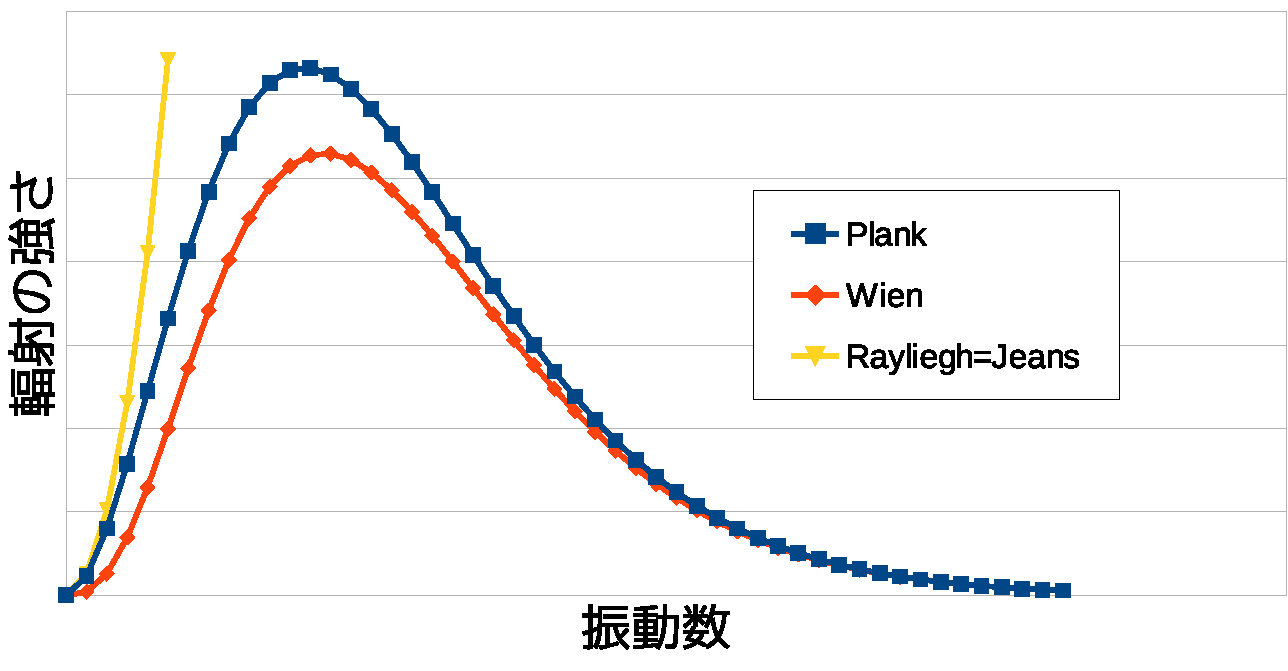
\includegraphics[keepaspectratio, width=7cm,height=4cm,clip]{BlackBoxRayleighWein.pdf}
                        \caption{各式による理論値と実験値の比較}
                        \label{fig:yu}
                    \end{center}
                \end{figure}

%       %======================================================================
%       %  Subsection
%       %======================================================================
        \subsection{プランクの式}
            プランク
                \footnote{
                    Max Karl Ernst Ludwig Planck (1858 - 1947),ドイツ
                }
            は,黒体放射の実験と一致する式を見出した.
            \begin{myshadebox}{プランクの式}
                プランクは黒体放射の強度 $u(\nu,\,T)$ と周波数 $\nu$ の の関係
                を表す式として,次式を提案した.
                    \begin{align}
                        u(\nu,\,T) = \frac{8 \pi}{{c}^{3}}
                                     {\nu}^{2}
                                     \frac{h \nu}{\exp\left( \frac{h \nu}{{k}_{B}T} \right) - 1}.
                    \end{align}

                $T$ は黒体の絶対温度,$\nu$ はそのときに放射される電磁波の周波数,$h$ はプランク定数,
                ${k}_{B}$ はボルツマン定数,$c$ は光速である.
            \end{myshadebox}

            この式は,$\nu$ が小さいときに($\nu \rightarrow 0$),レイリー$=$ジーンズの式に形を
            変える.また,$\nu$ が大きいときに($\nu \rightarrow \infty$),ウィーンの式になる.
            このことを,簡単に確認しておこう.

            \subsubsection{$1/({\e}^{x} -1)$ の極限}
            まず,次の関数の極限について知っておく必要がある.
            \begin{myshadebox}{$\displaystyle \frac{1}{\exp(x) - 1}$ の極限}
                以下の関数 $f(x)$ を考える.
                \begin{align}
                    f(x) = \frac{1}{\exp(x) - 1}
                \end{align}
                この関数は,極限に関する次の性質がある.
                \begin{align*}
                    \mbox{(1)} \quad \lim_{x \rightarrow 0} f(x) = \frac{1}{x} \quad , \qquad
                    \mbox{(2)} \quad \lim_{x \rightarrow \infty} f(x) = \frac{1}{\exp(x)}
                \end{align*}
            \end{myshadebox}

            この式の $x$ を,$x=h\nu/{k}_{B}T$ とすると,プランクの式の一部分になる.
            便宜上,一時的にその部分を,$X(\nu)$ と表そう.
            \begin{equation*}
                X(\nu) = \frac{h \nu}{\exp\left( \frac{1}{{k}_{B}T} \right) - 1 }
            \end{equation*}
            この時,以下の式が成り立つ.
            \begin{itemize}
                \item 低周波領域では,
                    $\displaystyle \lim_{\nu \rightarrow 0}      X(\nu) = \frac{{k}_{B}T}{h\nu}$ \\
                \item 高周波領域では,
                    $\displaystyle \lim_{\nu \rightarrow \infty} X(\nu) = \frac{1}{\exp\left(\frac{h\nu}{{k}_{B}T}\right)}$
            \end{itemize}

            \subsubsection{レイリー$=$ジーンズの式との関係}
            プランクの式は,この $X(\nu)$ を使うと,
            \begin{equation*}
                u(\nu,\,T) = \frac{8 \pi}{{c}^{3}} {\nu}^{2} (h \nu) X(\nu)
            \end{equation*}
            となる.
            低周波領域では,$X(\nu) = {k}_{B}T/h\nu$ であるから,
            \begin{align*}
                u(\nu,\,T) &= \frac{8 \pi}{{c}^{3}} {\nu}^{2} (h \nu) X(\nu) \\
                           &= \frac{8 \pi}{{c}^{3}} {\nu}^{2} (h \nu) \frac{{k}_{B}T}{h\nu} \\
                           &= \frac{8 \pi}{{c}^{3}} {\nu}^{2} {k}_{B}T
            \end{align*}
            と計算される.
            \begin{equation*}
                u(\nu,\,T) = \frac{8 \pi}{{c}^{3}} {\nu}^{2} {k}_{B}T
            \end{equation*}
            はレイリー$=$ジーンズの式に他ならない.

            \subsubsection{ウィーンの式との関係}
            高周波領域では,
            \begin{equation*}
                X(\nu) = \frac{1}{\exp\left(\frac{h\nu}{{k}_{B}T}\right)}
            \end{equation*}
            であるから,
            \begin{align*}
                u(\nu,\,T) &= \frac{8 \pi}{{c}^{3}} {\nu}^{2} (h \nu) X(\nu) \\
                           &= \frac{8 \pi h}{{c}^{3}} {\nu}^{3} \frac{1}{\exp\left(\frac{h\nu}{{k}_{B}T}\right)}
            \end{align*}
            ここで,$h=B$ とすれば,
            \begin{equation*}
                u(\nu,\,T) = \frac{8 \pi B}{{c}^{3}} {\nu}^{3} \frac{1}{\exp\left(\frac{B\nu}{cT}\right)}
            \end{equation*}
            となり,ウィーンの式に一致する.

%   %==========================================================================
%   %  Section
%   %==========================================================================
    \section{光の粒子性,電子の波動性}
%       %======================================================================
%       %  Subsection
%       %======================================================================
        \subsection{光は粒子としても振る舞う}
            電磁気学で学んだ通り,光は電磁波であり,従って「光は波である」と結論される.こ
            のことを,光は \textbf{波動性} の性質をもつという.
            しかし,後に示す \textbf{光電効果} という現象を観測すると,「光は波である」と
            いう主張と矛盾する部分が生じる.光電効果を観測する場合には,光は波動性ではなく
            粒子のような性質を示すのである.
            粒子のような性質のことは,光の \textbf{粒子性} とよばれる.今までの学習で常識
            的考えれば,波動性と粒子性は互いに相反する現象であり,物理現象がその性質として
            両方の性質を同時にもつものとは考えにくい.しかし,実際にそのような現象が,私達
            の馴染み深い「光」という物理現象がもっていることは事実であり,これを受け入れる
            必要がある.

%       %======================================================================
%       %  Subsection
%       %======================================================================
        \subsection{アインシュタインの光量子}
            エネルギーの変化は連続的なものではなく,離散的なものではないかとPlanckが提案をした.
            エネルギーが離散的に変化するとは,ある決まった値の整数倍の値しかとることができないということである.
            ある決まった値とは,
                \begin{align}
                    E=\nu h
                \end{align}
            である.
            アインシュタインはこのPlanckの提案を受けて,光電効果の理論的説明を与えた.アインシュタインは
            “光は粒子である”ということを仮定ば,光電効果を説明できることを示した.
                \begin{align}
                    E=h\nu
                \end{align}
            だが,
                \begin{align*}
                    \hbar := \frac{h}{2\pi}\;,\quad\omega:= 2\pi\nu
                \end{align*}
            を導入すれば,
                \begin{align}
                    E=\hbar\omega
                \end{align}
            と書ける.

            \being{memo}{$E=h\nu$}
                $E=h\nu$の左辺であるエネルギー$E$は粒子性を表している.そして右辺の$\nu$は波動性を表す.
                つまり、この式は粒子性と波動性を関係付ける式である。この式をもう少し詳しく見ていこう.
                エネルギー順位がmからnに変化したときのエネルギーを,${E}_{m \rightarrow n}$と書こう.
                そして,このときに放出される電磁波の振動数を${\nu}_{m \rightarrow n}$とする.
                この場合の関係式は,次のとおりになる.
                \[
                    {E}_{m \rightarrow n}=h{\nu}_{m \rightarrow n}.
                \]
                これを以下のように式変形してみる.
                \[
                    \frac{{E}_{m \rightarrow n}}{{\nu}_{m \rightarrow n}} = h.
                \]
                つまり,放出されるエネルギーとそのときに発生する電磁波の比が$h$という一定の値(プランク定数)に
                なるということである.mとnは任意の自然数である
                    \footnote{
                        ただし,ここではm$>$nを想定している.
                    }.
                
            \end{memo}

%       %======================================================================
%       %  Subsection
%       %======================================================================
        \subsection{光電効果}
            レーナルト
                \footnote{
                    Philipp Eduard Anton von Lenard (1862 - 1947),ハンガリー
                }
            は光電効果を実験的に発見した.光電効果とは,簡単にいえば,金属に光を
            照射したときに,金属表面から電子が飛び出してくる現象をいう.
                        \begin{figure}[hbt]
                            \begin{center}
                                \includegraphicsdefault{kouden_kouka_image_1.pdf}
                                \caption{光電効果のイメージ}
                                \label{fig:kouden_kouka_image_1}
                            \end{center}
                        \end{figure}

            レーナルトが実験で得た光電効果の性質は3つある.すなわち,\\
                \begin{itembox}[l]{光電効果の性質}
                    \begin{enumerate}
                    \item 光電効果が起こるためには,金属表面に照射する光の周波数  $\nu$  が,
                            その金属に特有なある一定の周波数 $\nu_{0}$ より
                            大きくなければならない.この $\nu_{0}$ を \textbf{光電限界周波数} という.
                            $\nu < \nu_{0}$ だと,つまり,照射する光の周波数が $\nu_{0}$ 以下であると,
                            光電効果は起こらない.逆に,$\nu > \nu_{0}$ で
                            れば,つまり,照射する光の周波数が $\nu{0}$ より大きければ,どんなに弱い光でも,
                            光電効果は起こる.
                    \item 光電効果によって金属表面から飛び出る電子のエネルギー $E$ は,
                            光の強さに無関係であり,照射する光の周波数 $\nu$ のみ
                            によって決まる.$\nu > \nu_{0}$ の場合に,照射する光の周波数 $\nu$ と
                            飛び出す電子のエネルギー $E$ の関係は
                            \begin{align}\label{eq:Light_eq1}
                                E = h\nu -h\nu_{0}
                            \end{align}
                            で与えられる.ここに,$h$ はPlanck定数である.
                    \item 光の強さを大きくすると,金属表面から飛び出す電子の個数が増える.
                            しかし,ここの電子のエネルギーは変わらず,式(\ref{eq:Light_eq1})によって決まる.
                    \end{enumerate}
                    (阿部 龍蔵 [著],『量子力学入門』,岩波書店,2004,p31-32 を参照した.)
                \end{itembox}\\

            光電効果の関係式(\ref{eq:Light_eq1})の $h\nu_{0}$ は定数であるので,これを $W$ とおく($W=h\nu_{0}$).
            この $W$ は金属固有の値であり,各金属で異なった値をとる.$W$ を \textbf{仕事関数} という.
            また,光電効果によって金属表面から飛び出した電子のエネルギーは,もはや金属陽イオンからのクーロン力の影響
            がなく,ポテンシャルを無視できるので,運動エネルギーのみによって表現できる.飛び出す
            電子の速度を $v$,質量を $m_{e}$ としたとき,運動エネルギーは $E=(1/2)mv^{2}$ である.
            以上から,光電効果の関係式(\ref{eq:Light_eq1})は以下のように表現することもできる.
                                    \begin{align}\label{eq:Light_eq2}
                                        E &= h\nu -h\nu_{0} \notag \\
                                        \Leftrightarrow \quad \frac{1}{2}m_{e}v^{2} &= h\nu - W
                                    \end{align}
            これを,\textbf{アインシュタインの光電方程式} という.

            \begin{figure}[hbt]
                \begin{center}
                    \includegraphicsdefault{kouden_kouka_image_2.pdf}
                    \caption{光電効果(光は粒子だ!)}
                    \label{fig:kouden_kouka_image_2}
                \end{center}
            \end{figure}

%       %======================================================================
%       %  Subsection
%       %======================================================================
            \subsection{振動現象と等速円運動}
                振動現象と等速円運動についての復習をする.

                                \begin{figure}[hbt]
                                    \begin{tabular}{cc}
                                        \begin{minipage}{0.5\hsize}
                                                        \begin{center}
                                                            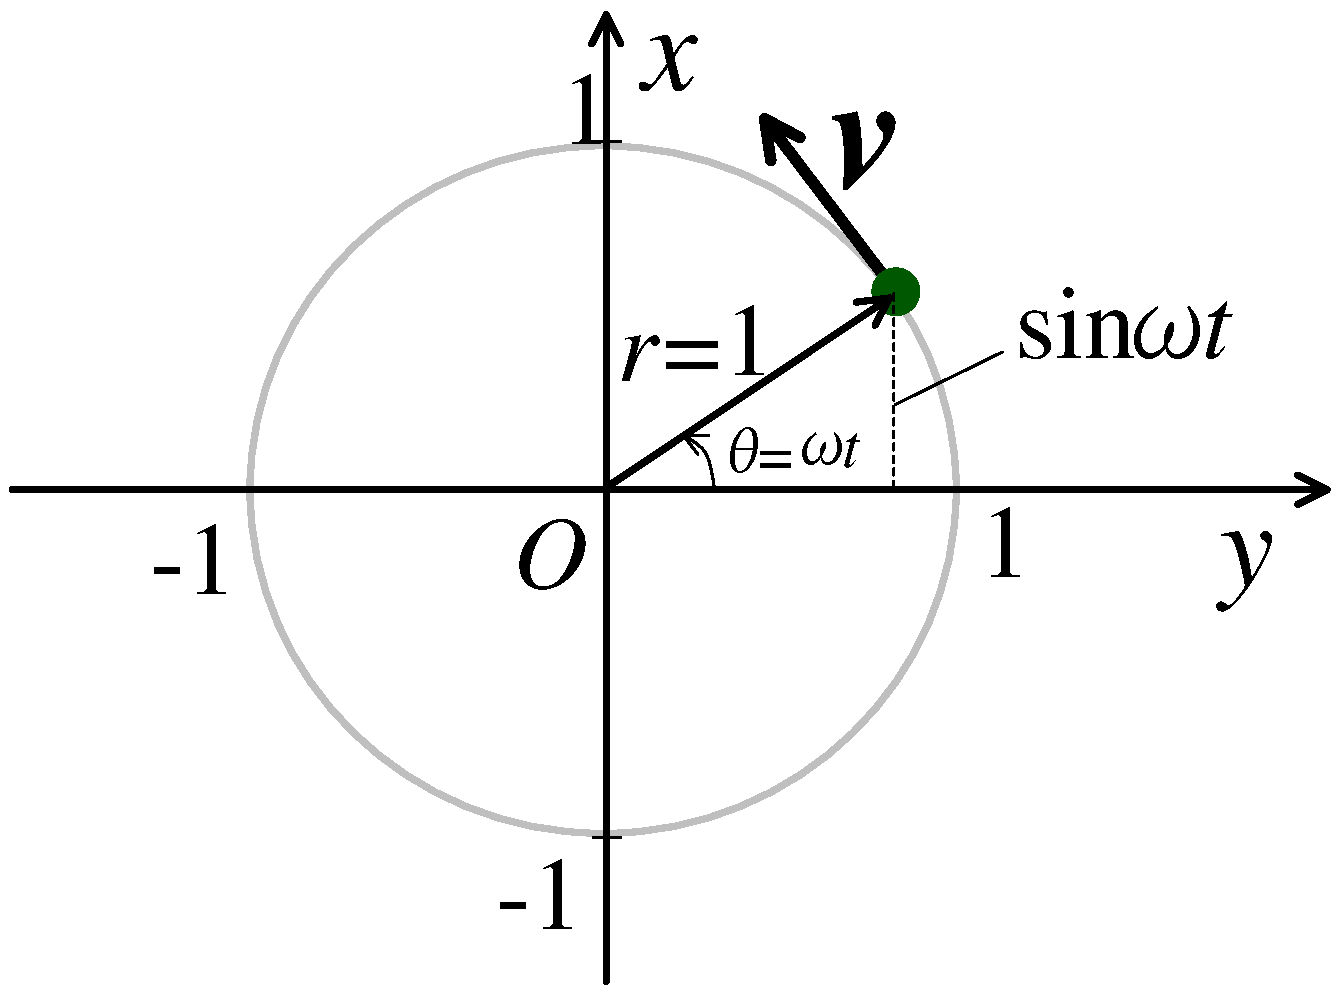
\includegraphics[keepaspectratio, width=3.4cm,height=4.2cm,clip]{enubdou2.pdf}
                                                            \caption{\ 等速円運動の関係}
                                                            \label{fig:enubdou2}
                                                        \end{center}
                                        \end{minipage}
                                        \begin{minipage}{0.5\hsize}
                                                        \begin{center}
                                                            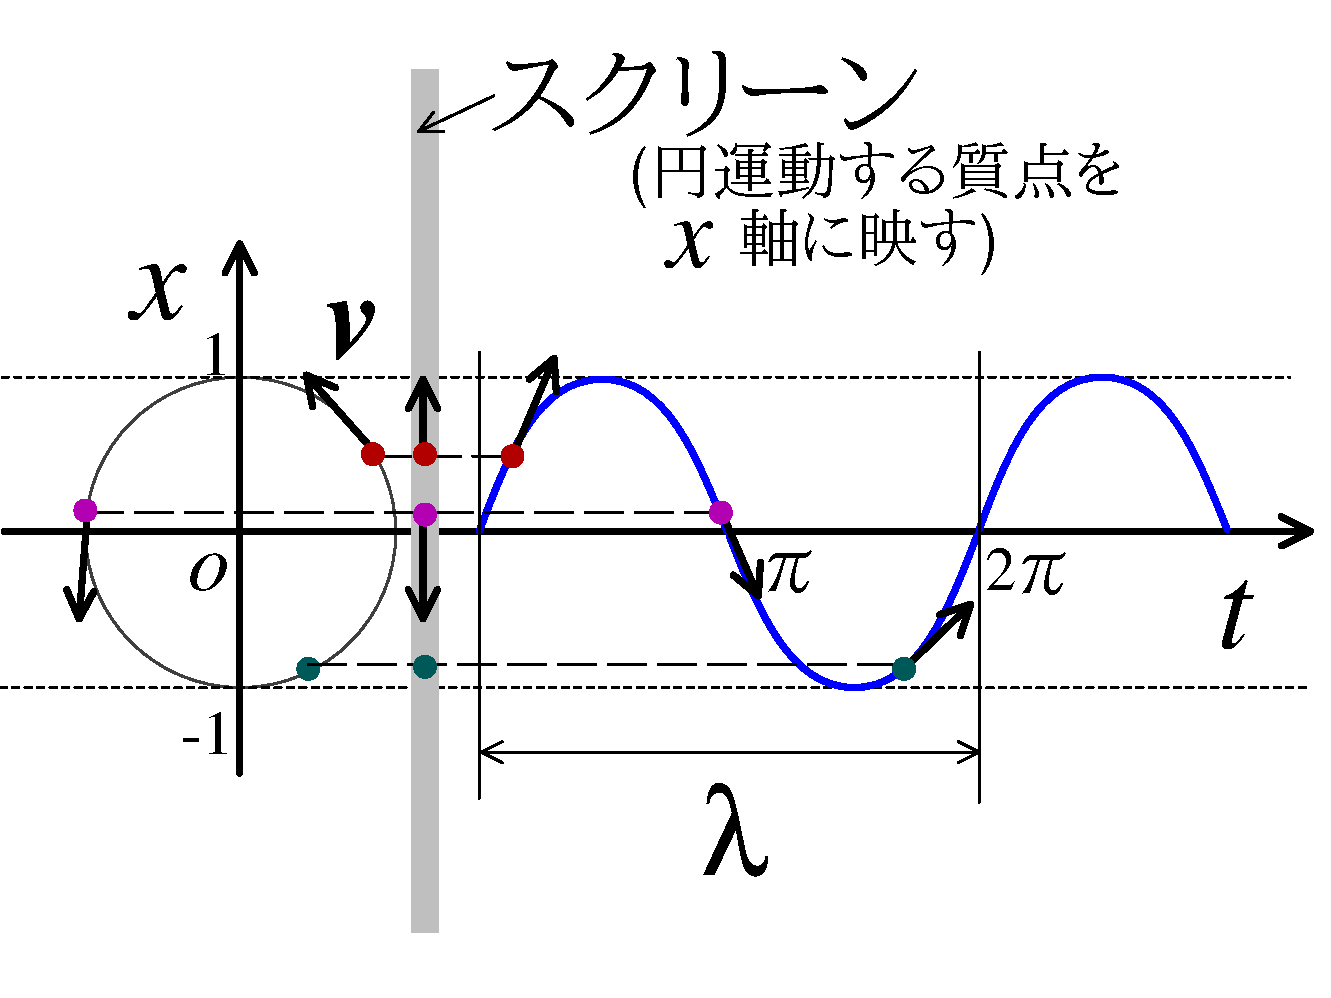
\includegraphics[keepaspectratio, width=3.4cm,height=4.2cm,clip]{enundou.pdf}
                                                            \caption{\ 単振動と等速円運動の関係}
                                                            \label{fig:enundou}
                                                        \end{center}
                                        \end{minipage}
                                    \end{tabular}
                                \end{figure}

                        まず,質点の等速円運動を考える.図\ref{fig:enubdou2}参照.半径が1である円を \textbf{単位円} という.
                        単位円の円周の長さ
                                    \footnote{
                                    半径 $r$ の円の円周の長さは $2\pi r$ である.
                                    }
                        は,$2\pi$ である.だから,この質点が単位円上を回転する速度は,
                        質点が単位円を一周するまでの時間 $T$ で円周の長さ $2\pi$ を割ればよい.
                        回転の速さのことを \textbf{角速度} ということにすれば,
                        角速度 $\omega$ は以下のように定義できる.
                            \begin{align}\label{eq:kakushuhasuu}
                                \omega=\frac{2\pi}{T}
                            \end{align}

                        さて,図\ref{fig:enundou}により,
                        質点の等速円運動の $x$ 成分だけを見ると,質点は $x$ 軸上を
                        単振動しているように見える.なぜなら,$x=\sin\omega t$ の関係があるからである.
                        この意味で,角速度は \textbf{角周波数}
                                    \footnote{
                                    定義によれば,単位円(半径 $r=1$ の円)を周期 $T=2\pi$ で
                                    一周すると,角速度が $\omega =1$ となる.
                                    }
                        とよばれることもある.
                        質点が単位円を1周するまでの時間 $T$ は単振動における \textbf{周期} に対応している
                        ことも明らかである.これからは単振動のほうを主に考えるので,
                        $\omega$ を角周波数と書き,$T$ を周期と書くことにする.


                        ところで,振動の周期 $T$ と \textbf{周波数}
                        \footnote{
                        周波数とは1[s]間における,質点の振動の回数である.
                        }
                        $\nu$ の間には,
                            \begin{align}
                                T=\frac{1}{\nu}\, \quad\left(\Leftrightarrow  \nu=\frac{1}{T} \right)
                            \end{align}
                        の関係がある.式(\ref{eq:kakushuhasuu})にこの関係式を考慮すば,
                            \begin{align}
                                \omega=2\pi\nu
                            \end{align}
                        を得る.

%           %==================================================================
%           %  Subsubsection
%           %========================s==========================================
%            \subsubsection{}


%===================================================================================================
%  Chapter : 量子力学
%  説明    : 量子力学入門
%===================================================================================================
\chapter{量子力学}
%   %-----------------------------------------------------------------------------------------------
%   %  Input
%   %    File Name : PhysNote_QM_Main.tex
%   %    説明      : 量子力学
%   %-----------------------------------------------------------------------------------------------
        %   %==========================================================================
%   %  Section
%   %==========================================================================
    \section{量子力学の教科書}
        \subsection{説明方法}
            多くの量子力学の教科書は次の2つの種類のうちのどちらかである.
            \begin{itemize}
                \item 歴史的なこと(量子力学の由来)から説明していくもの
                \item 量子力学の本質を,体系立てて説明するもの
            \end{itemize}
            以下で,その長所と短所を説明した後に,このノートの量子力学の
            学習方針を示す.

        \subsection{歴史的記述から入る教科書}
            \begin{mysmallsec}{長所}
                歴史的なことから記述されている教科書は,学習の動機とか,量子力学の必要
                性とかをつかむことができる.
            \end{mysmallsec}

            \begin{mysmallsec}{短所}
                本論に入るまでには歴史的記述が長く続くことになるので,
                量子力学の本論に到達するまでに時間が掛かってしまう.
                志が低いと,本論に入る前に挫折してしまうことがある
                \footnote{
                    単位取得のみを目的とする大学生や,
                    趣味で勉強しようとする人にとっては,つらいのだ.
                    (私は,昔は前者であり,今は後者である)
                }
            \end{mysmallsec}

        \subsection{いきなり体系から入る教科書}
            \begin{mysmallsec}{長所}
                量子力学の本質から入る教科書は,はじめから本質から入るので時間は掛からない.
            \end{mysmallsec}

            \begin{mysmallsec}{短所}
                量子力学の必要性がよくつかみにくくなってしまう.
                また,量子力学特有の抽象的な概念が容赦なく押し付けられるため,
                お手上げ状態になる可能性が高い.
            \end{mysmallsec}

        \subsection{このノートの学習方針}
            このノートは,量子力学を以下の手順で学習する.
            \begin{mysmallsec}{step1. 数式の少ない入門書を読む}
                \begin{itemize}
                \item ブルーバックスなど一般向けの量子力学の入門書が多く出版されている.
                      まず,これにより量子力学の概要をつかむ.
                \item この段階ではWebを参照しないほうが良い.
                      なんの学習をするにしても,Webからの情報を得ることは不可欠だが,
                      誤っている記述も散見されるため,注意が必要.
                      気になって見たとしても,信じこまないように.
                \end{itemize}
            \end{mysmallsec}

            \begin{mysmallsec}{step2. 易しい入門書を読む}
                \begin{itemize}
                \item 易しく記述されている量子力学の教科書を読む.
                      数式を用いた説明がなされてはいるが,
                      本当の初学者向けに書かれている独習書を選ぶ.
                      "高校数学だけでわかる"的なものがいい.
                \end{itemize}
            \end{mysmallsec}

            \begin{mysmallsec}{step3. 標準的な教科書を読む}
                \begin{itemize}
                \item 最後に,原島や砂川,小出,シッフなどの,標準的な教科書を読む.
                      教科書を2,3冊つ選び学習したいところだ.
                      ただし,学習の軸とする教科書を1つに定めてこれを基本に学習を進め,
                      他は副読的に読むこと.2,3冊を同時に読み込もうとしないこと.
                      読み込むのは1冊で十分.
                      基本とする教科書で,内容が足りなかったり,わかりにくい記述が
                      あった場合に,副読用の教科書を参照するという方法がいい.
                \item 物理学の解説Webサイトの参照も有用である.
                      ただし,その記述を読む際には,批判的であること.
                      Webの情報の多くは,他人の検閲が行われないため,
                      執筆者の個人的なの考えや感想である.
                      大学の教授によって,その大学の名(研究室名)の下に書かれていれば,
                      その内容の信頼性は高いが,個人サイトの閲覧は要注意である.
                \item さらに,この段階で,量子力学の学習と並行して,\textbf{解釈問題} など
                      の哲学的問題にも触れておきたい.解釈問題は理解しなくともよいが,
                      理論の基本思想が複数あるということを知っておくべきである.
                      この解釈問題を追っていくと,\textbf{多世界解釈} といった話題に
                      つながっていく.
                \item また,\textbf{因果律の捉え直しが必要} であったり,観測行為が
                      実験結果に強く影響を与えてしまうと問題(\textbf{観測問題})が
                      あることを認識しておきたい.
                      観測問題は量子力学の基本原理の1つである \textbf{不確定性原理} に
                      関連した問題だ.
                \end{itemize}
            \end{mysmallsec}

            \begin{mysmallsec}{step4. もっと難しい教科書を読む}
                \begin{itemize}
                \item ディラックやノイマン,ランダウ$=$リフシッツなどの,
                      難しい教科書に挑戦する.あるいは,本屋や図書館で,
                      その内容をチラ見する.
                \item 量子力学の難しさを痛感することが目的だ.
                      教科書の内容を理解することが目的ではない.
                \item 万が一,更に学習を進めたいという向学心に目覚めた場合に,
                      挑戦すべき教科書を予め定めておくのもよいことだと思う.
                      標準的な教科書を読んで,量子力学をわかった気になってはいけない.
                \end{itemize}
            \end{mysmallsec}

        \subsection{使用する教科書}
            このノートにおける量子力学の教科書として,以下を使用する.
                \begin{itemize}
                    \item (step1) J.C.ポーキングホーン 著,宮崎 忠 訳,『量子力学の考え方』,講談社ブルーバックス
                    \item (step1) 山田 克哉 著,『量子力学のからくり --- 「幽霊波」の正体』,講談社ブルーバックス
                    \item (step2) 竹内 淳 著,『高校数学でわかるシュレーディンガー方程式』, 講談社ブルーバックス
                    \item (step2) 都筑 卓司 著,『なっとくする量子力学 』,講談社
                    \item (step3) 中嶋 貞雄 著,『量子力学 \I / \II 』(物理入門コース5/6),岩波書店
                    \item (step3) 前野 晶弘 著,『よくわかる 量子力学』,東京図書
                    \item (step3) 佐川 弘幸,清水 克多郎 著,『量子力学(第2版)』,丸善
                    \item (step3) コリン・ブルース 著,和田 純夫 訳,『量子力学の解釈問題』,講談社ブルーバックス
                \end{itemize}

%   %==========================================================================
%   %  Section
%   %==========================================================================
    \section{量子力学での運動方程式}
        \subsection{はじめに}
            上に書いたように,原子のような非常に微小な世界では,ニュートン力学が成り立たなくなってしまう.つま
            り,原子や電子,光子の運動はニュートンの運動方程式では表現できない.これは実験事実であって,認める
            よりしかたがない.しかし,ニュートンの運動方程式に従わないからといって,デタラメに運動しているわけ
            ではない.何か“別の運動法則”に従って運動しているのである.

        \subsection{量子力学での運動方程式}
            \subsubsection{運動方程式は2種類の表現方法がある}
            では,どのような運動法則に従っているのだろうか.この疑問に答えを見つけたのが,ハイゼンベルクである.
            シュレディンガーもハイゼンベルクと独立に,一年遅れだが答えを見つけている.
            ハイゼンベルクの見つけた運動方程式は,行列という数学の形式を用いて表現されるものだった.
            発見当時は,科学者は行列という形式に不慣れだったため,ハイゼンベルクの
            発見はあまり目立ったものではなかった.ハイゼンベルクが行列形式の運動方程式を発見した一年後に,
            シュレディンガーは偏微分方程式を用いた形式の運動方程式を発見した.当時の科学者にとって,偏微分方程式は
            研究に欠かせいない道具であったので,シュレディンガーの発見した方程式はすぐに有名になった.
            もちろんハイゼンベルクの発見した運動方程式が間違っていたのではない.
            ハイゼンベルクとシュレディンガーが発見した2つの運動法則
            は全く同等であることは,シュレーディンガーによって証明されている.違いは,単に,数学形式だけである.
            なので,量子力学には2種類の記述方式があるということになる.
            一つは,ハイゼンベルクの行列を用いた表現方法で,\textbf{行列力学} とよばれ,
            その方程式は \textbf{ハイゼンベルク方程式} といわれる.
            もう一つは,シュレーディンガーの偏微分方程式による表現方法で,\textbf{波動力学} とよばれ,
            その方程式は \textbf{シュレーディンガー方程式} といわれる.

            行列力学は,波動力学に比べると,抽象的である.量子力学の体系を構築する場合には,
            行列力学が有用である.しかし,実際に生じる個々の物理現象を解析するには,波動力学が
            便利である.個人的に,行列よりも偏微分方程式のほうが扱いなれているので,
            シュレディンガー方程式を先に学習する.数学的テクニックや学習のしやすさを考えても,
            まずはシュレーディンガー方程式から量子力学へ入門する方がよいと思う.実際に,
            そういう教科書のほうが圧倒的に多く出版されている.

            \subsubsection{シュレーディンガー方程式の導入}
            \begin{mysmallsec}{方程式は論理的に導けない}
            光子や電子などの量子は,全てシュレディンガー方程式に従っている
                \footnote{
                    相対論的効果が無視できない場合は,シュレディンガー方程式を拡張した,ディラックの運動方程式で
                    記述される.しかし,ここでは,相対論的効果が無視できるような状況を仮定する.
                }.

            シュレディンガー方程式は,ニュートン方程式と同様に,論理的考察によって導き出すことはできない.だか
            らといって,シュレディンガー方程式はこうだ!!と強要されても,納得できない.
            しかし,シュレディンガーの推論を辿ることは可能である.
            \end{mysmallsec}

            \begin{mysmallsec}{自由粒子の一次元の運動}
            以下では,非常に微小で電荷等をもたない,純粋な自由粒子の一次元の運動を考える.自由粒子は,ポテ
            ンシャルエネルギーをもっておらず,自身のもつ速度による運動エネルギーのみをもっていると仮定する
            .自由粒子にはド$\cdot$ブロイの \textbf{物質波} という波の性質がある.
            この物質波を $\psi(x,\,t) $ と表す.$\psi(x,\,t) $ は以下のような波動関数で記述されると仮定する.
                \begin{align}\label{e_bussituha}
                    \psi(x,\,t) = A\e^{i\left( \frac{p}{\hbar}x-\frac{E}{\hbar} t\right)}.
                \end{align}
            ここに,$A$ は定数で,波動関数の振幅である.$x$ 軸は自由粒子の運動方向にとる.この $\e$ は指数
            関数である.なぜこの関数が自由粒子の物質波を表現するかについてはよく分からないが,こう仮定する
            と,実験結果とよく整合が取れるのである.とりあえず,ここでは,波動関数の意味を考えず,これを仮
            定した上で,話を進めていこう.
            \end{mysmallsec}

            \begin{mysmallsec}{量子力学における,運動量とエネルギー}
            波動関数(\ref{e_bussituha})の波数 $k$ と,角周波数 $\omega$ はそれぞれ,ド$\cdot$ブロイの関係から,
            運動量 $p$ とエネルギー $E$ で表現できる.つまり,$k=p/\hbar$,$\omega=E/\hbar$ の関
            係によって波動関数(\ref{e_bussituha})は
                \begin{align}\label{e_bussituha_2}
                    \psi(x,\,t) = A\e^{i\left( kx -  \omega t\right)}
                \end{align}
            と書き表せる.波動関数の変数は位置 $x$ と時間 $t$ である.この波動関数 $\psi(x,\,t)$ が満たし
            ている方程式を考えるため
                \footnote{
                    運動量に対応する演算子と,エネルギーに対応する演算子を知りたいから.
                },
            その独立変数 $x,\,t$ でそれぞれ偏微分する.

            まず,波動関数 $\psi(x,\,t)$ を位置 $x$ で偏微分して,
                \begin{align}\label{hadoukansu_p}
                    \frac{\rd \psi(x,\,t)}{\rd x}
                        &= i\frac{p}{\hbar}A\e^{i\left( kx -  \omega t\right)} \notag \\
                        &=i\frac{p}{\hbar}\psi(x,\,t) \notag \\
                    \therefore \quad
                    \frac{\rd \psi(x,\,t)}{\rd x}
                        &= i\frac{p}{\hbar}\psi(x,\,t).
                \end{align}

            次に $\psi(x,\,t)$ を時間 $t$ で偏微分して
                \begin{align}\label{hadoukansu_e}
                    \frac{\rd \psi(x,\,t)}{\rd t}
                        &= -i\frac{E}{\hbar}A\e^{i\left( kx -  \omega t\right)} \notag \\
                        &=-i\frac{E}{\hbar}\psi(x,\,t) \notag \\
                    \therefore \quad
                    \frac{\rd \psi(x,\,t)}{\rd t}
                        &= -i\frac{E}{\hbar}\psi(x,\,t).
                \end{align}

            そして,式(\ref{hadoukansu_p}),(\ref{hadoukansu_e})をそれぞれ $p$,$E$ について解いて,
                \begin{align*}
                    p\psi(x,\,t) &= -i\hbar\frac{\rd }{\rd x}\psi(x,\,t) \\
                    E\psi(x,\,t) &=  i\hbar\frac{\rd }{\rd t}\psi(x,\,t)
                \end{align*}
            を得る.ここで,計算中に分母に現れる虚数単位 $i$ は,式の見やすさを考えて有理化した,
            両辺に $\psi(x,\,t)$ がかかるように記述したのは,運動量に対応する演算子と,エネルギーに対応す
            る演算子を知りたかったからである.この式を見ると,運動量 $p$ とエネルギー $E$ は,次のように対
            応していることがわかる.
                \begin{align}
                    p &\Leftrightarrow  -i\hbar\frac{\rd }{\rd x}. \\
                    E &\Leftrightarrow   i\hbar\frac{\rd }{\rd t}.
                \end{align}
            \end{mysmallsec}

            \begin{mysmallsec}{エネルギー保存則が成立すると仮定する}
            運動量 $p$ とエネルギー $E$ の関係を記述する式として,エネルギー保存の法則がある.
            ここで,何らかのポテンシャル(電位でも重力ポテンシャルでもなんでもいい)を加えて,
            これを $V(x,\,t)$ として,
                \begin{equation*}
                    E = \frac{p^{2}}{2m} + V(x,\,t).
                \end{equation*}
            ここに,$m$ は質量である.

            量子力学でもエネルギー保存の法則を満たしているはずである.
                \footnote{
                    古典力学のエネルギー保存の法則は,反証的な実験結果が報告されていないという意味で,
                    今までに破られたことはない.これは,量子力学を適用すべき微視領域の実験でも同じである.
                    実際,時間の対称性から,ネーターの定理によって,エネルギー保存則が導かれる.

                    しかし,時間とエネルギーの不確定性原理によると,エネルギー保存則が破られる
                    瞬間がある.微小時間内ではエネルギーの値が1つの値に定まらず,エネルギーが
                    突然増えたり減ったりする時間があるのだ.このエネルギー保存則の敗れは,
                    量子力学的な微視的範囲でのみ発生し,マクロには現れない現象である.

                    ついでに,もっと言うと,時間も不確定になるために,量子力学的領域では,
                    因果関係が曖昧になっている.
                }
            として,運動量 $p$ とエネル
            ギー $E$ を上で得た対応する演算子に置き換えて,
                \begin{equation*}
                    i\hbar\frac{\rd }{\rd t}
                        = \frac{1}{2m}\left( i\hbar\frac{\rd }{\rd x} \right)^{2} + V(x,\,t).
                \end{equation*}
            整理しよう.
            \begin{equation*}
                i\hbar\frac{\rd }{\rd t}
                    = -\frac{\hbar^{2}}{2m}\frac{\rd^{2}}{\rd x^{2}} + V(x,\,t).
            \end{equation*}
            \end{mysmallsec}

            \begin{mysmallsec}{演算子の導入}
            形式的に \textbf{ハミルトニアン演算子} というものを導入してみよう.その記号として,
            $\hat{H}_{x}$ を用いることにする
                \footnote{
                    ただ,注意したいのは,量子力学でのハミルトニアン演算子は,
                    解析力学でのハミルトニアン $H$ とは全く別物であるということである.しかし,概念的に量
                    子力学のハミルトニアン演算子は,解析力学のハミルトニアン $H$ をヒントに導入されている
                    ので,似たような記号を使いたいというもある.そのため,$\hat{H}$ の$\hat{}$ (「ハット」
                    と読む)はそれらを区別するためにつけてある.

                    また,下添え字の $x$ は, いまは $x$ 軸方向だけしか扱っていないことを明示するためにつけた.
                    空間の3次元を考えるときは添え字を書くことはせず,単に $\hat{H}$ と記述する.
                }.

            解析力学で学んだハミルトニアンは,系の全エネルギーと等しかった.
            今の場合,ハミルトニアンそのものではなく,演算子的性質を持つハミルトニアン演算子である.
            これらを区別するために,演算子のほうには,文字の頭に $\hat{}$ をつけることにしよう.
            つまり,
                \begin{align}
                    \hat{H}_{x} = -\frac{\hbar^{2}}{2m}\frac{\rd^{2}}{\rd x^{2}} + V(x,\,t).
                \end{align}

            さらに,\textbf{エネルギー演算子} も同様に導入しよう.エネルギー演算子の記号は $\hat{E}$ とい
            う記号をつかう.
                \begin{align}
                    \hat{E} = i\hbar\frac{\rd }{\rd t}.
                \end{align}
            すると,形式的にと $\hat{H}_{x} = \hat{E}$ と書ける
                \footnote{
                    右辺と左辺を入れ替えてしまった.量子力学の教科書を見ると,
                    左辺にハミルトニアン演算子 $\hat{H}$,右辺にエネルギー演算子 $\hat{E}$ を書いている.
                    ここではそれに習うことにした.
                }.
            \end{mysmallsec}

            \begin{mysmallsec}{シュレーディンガー方程式の完成}
            しかしこの演算子の関係式は,物理的に何も意味しない.この演算子は,波動関数 $\psi(x,\,t)$ に作
            用させて始めて運動方程式の意味をなす.従って,
                \begin{align}\label{eq:Schrding_eq}
                    \hat{H}_{x} \psi(x,\,t) = \hat{E} \psi(x,\,t)
                \end{align}
            を得る.この式(\ref{eq:Schrding_eq})が \textbf{シュレディンガー方程式} である.
            \end{mysmallsec}

            \begin{mysmallsec}{3次元へ拡張}
            もちろん,$x$ 軸の一方向だけでなく,これらは簡単に3次元空間に拡張できる.$y$,$z$ 方向にも同様
            に考えられる.その場合,シュレディンガー方程式は次のように記述される.
                \begin{align}\label{eq:Schrding_eq_3d}
                    \hat{H} \psi(\br,\,t) = \hat{E} \psi(\br,\,t).
                \end{align}
            \end{mysmallsec}

            \begin{mysmallsec}{一言メモ}
            ここで得たシュレディンガー方程式(\ref{eq:Schrding_eq_3d})は時間を含むものであり,
            最も一般的なものである.ここではあたかも方程式を導いたように見えてしまうが,
            実はそうではない.物質が従うとする波動関数 $\psi(x,\,t)$ が天下り的に与えられていて,
            その信憑性に関する言及は全くない.

            同じ方程式ではあるが,ハミルトニアン演算子とエネルギー演算子を明示したシュレディンガー方程式を
            以下に書いておこう.先ほどの $\hat{H}$,$\hat{E}$ を具体的に記述しただけである.
                \begin{align}\label{eq:Schrding_eq2}
                    -\frac{\hbar^{2}}{2m}\biggl\{
                    \frac{\rd^{2}}{\rd x^{2}} + \frac{\rd^{2}}{\rd y^{2}} + \frac{\rd^{2}}{\rd z^{2}}
                    + V(\br,\,t) \biggr\} \psi(\br,\,t) = i\hbar\frac{\rd }{\rd t} \psi(\br,\,t).
                \end{align}
            \end{mysmallsec}

%       %======================================================================
%       %  Subsection
%       %======================================================================
            \section{対応原理}
                シュレディンガー方程式は
                解析力学における,ハミルトニアンとエネルギーの関係
                から推察される方程式である.\textbf{
                シュレディンガー方程式は論理的に
                導かれる方程式ではなく,
                経験によって得られる方程式である}.
                しかし,この方程式で多くの物理現象を
                説明することができ,それに加えて,この方程式を満たさない現象が
                確認されていないことから,シュレディンガー方程式
                は物理的に正しい方程式であるといってよい.

                古典力学(解析力学)では,
                ハミルトニアン $H$ は座標変数 $(x,\,y,\,z)$ と正準運動量 $(p_{x},\,p_{y},\,p_{z})$ と時間 $t$ の
                関数であり,
                \begin{align}
                  H=H(x,\,y,\,z,\,p_{x},\,p_{y},\,p_{z},\,t)
                \end{align}
                と書かれる.ハミルトニアンは,エネルギー $E$ と等しく,
                \begin{align}
                  H(x,\,y,\,z,\,p_{x},\,p_{y},\,p_{z},\,t)=E
                \end{align}
                である.

                量子力学における
                シュレディンガー方程式は
                ハミルトニアン $H$ の正準運動量 $(p_{x},\,p_{y},\,p_{z})$ とエネルギー $E$ を
                演算子に置き換える(この機械的な置換えのことを \textbf{対応原理} とよぶ).置き換えの際の
                対応は以下の通り.
                    \begin{myshadebox}{対応原理}
                      運動量演算子 $\hat{p}_{x},\,\hat{p}_{y},\,\hat{p}_{z}$ と
                      エネルギー演算子 $\hat{E}$ は,
                      運動量 ${p}_{x},\,{p}_{y},\,{p}_{z}$ とエネルギー $E$ に対して,
                      以下のうように対応させる.
                        \begin{align}
                          p_{x}\, &\rightarrow  \hat{p}_{x}:=-i\hbar\frac{\rd}{\rd x}\,, \\
                          p_{y}\, &\rightarrow  \hat{p}_{y}:=-i\hbar\frac{\rd}{\rd y}\,, \\
                          p_{z}\, &\rightarrow  \hat{p}_{z}:=-i\hbar\frac{\rd}{\rd z}\,, \\
                          E    \, &\rightarrow  \hat{E}:=i\hbar\frac{\rd}{\rd t}
                        \end{align}
                    \end{myshadebox}

                矢印の左側が運動量 $\bp$ と エネルギー $E$ である.左側の
                アルファベットの上に $\hat{}$ が上についた文字は,演算子を意味すると約束しよう
                  \footnote{
                    $\bp$ と $E$ に対して深い関係がありそうなので,アルファベットはその関連する
                    ものを使用しておきたいということと,同時に,演算子であることを示す必要があるので,
                    このような表記になっている.$\hat{}$ の有無で意味が全く異なるので,注意すること.
                  }.

                そして,置き換えた演算子をそれぞれ波動関数 $\psi(x,\,t)$ に作用させて,次式を得る.
                        \begin{myshadebox}{時間を含むシュレディンガー方程式}
                          シュレディンガーの式(\ref{eq:shrdngr_tin})を,\textbf{時間を含むシュレディンガー方程式} という.

                            \begin{align}\label{eq:shrdngr_tin}
                              \hat{H}\left(x,\,y,\,z,\,\hat{p}_{x},\,\hat{p}_{y},\,\hat{p}_{z},\,t\right)\psi(x,\,t)=\hat{E}\psi(x,\,t)
                            \end{align}
                        \end{myshadebox}

%   %==========================================================================
%   %  Section
%   %==========================================================================
    \section{電子の速度}

%       %======================================================================
%       %  Subsection
%       %======================================================================
            \subsection{間違った考察}
                電子の速度を,量子力学の関係式から,
                どう表されるかを,考えてみよう.
                量子力学では,次の関係式が成り立つことが
                要求される.すなわち,
                    \begin{align}
                        p   =   \frac{h}{\lambda }.  \\
                        E   =   h\nu.
                    \end{align}

                さて,波動の速度の式を思い出してみると,
                    \begin{align}
                        v  =  \nu \lambda.
                    \end{align}
                量子力学が要請する2つの式より,$\lambda = h/p$,
                $\nu = E/h$ を上式に代入すると,
                    \begin{equation*}
                        v = \frac{E}{h} \frac{h}{p} = \frac{E}{p}
                    \end{equation*}
                となる.これを $E$ について解いてみる.
                    \begin{equation*}
                        E = pv.
                    \end{equation*}
                ところで,シュレディンガー方程式の考察でも用いたように,
                量子力学でも,運動エネルギーの式 $E = p^{2}/2m$ は有効である.
                これを上式 $E$ に代入すると,
                    \begin{equation*}
                        \frac{p^{2}}{2m} = pv.
                    \end{equation*}
                整理すると,
                    \begin{equation*}
                        p = 2mv.
                    \end{equation*}
                この式は,今まで考えてきた,運動量の式 $p=mv$ と
                異なっている.量子力学的には,$p=mv$ が間違っていて,
                $p=2mv$ が成立しているのだろうか.
                次の項目で,このことについて考えてみよう.

%       %======================================================================
%       %  Subsection
%       %======================================================================
            \subsection{電子の群速度}
                実は,波動の速度を考えるときには,その速度が2種類
                あることを忘れてはいけない.波動のもつ速度には,
                \textbf{位相速度} と \textbf{群速度} の2つがある.
                ここで考えていたのは,位相速度の方であった.
                しかし,波動の運動量を考えるときには,
                群速度を考えないといけない.


%       %======================================================================
%       %  Subsection
%       %======================================================================
            \subsection{電子の有効質量}
                電子を量子力学的にみた場合,粒子の性質だけでなく,
                波動現象も考慮する必要がある.量子力学では,
                電子のもつ運動量 $\bp$ とエネルギー $E$ は,
                それぞれ,波数 $\bk$ と各周波数 $\omega$ と
                次の関係がある.
                    \begin{align}
                        \bp  &=  \hbar \bk    \\
                        E     &=  \hbar \omega
                    \end{align}
                この関係から,電子の運動の速度を考えてみよう.この場合,
                電子の速度とは,位相速度ではなく,群速度で考える必要がある.

                ポテンシャルが存在しない場合は,
                電子は何とも相互作用しないから,質点と同じように扱うことができるが,
                固体中の電子は,固体原子と相互作用をしてしまうので,質点と同じように考えることができない.
                電子が波の性質の有することを考慮しているためである.
                電子のもつエネルギー $E$ は,
                エネルギーに関するアインシュタインの関係式により,
                   \begin{align}
                        E=\hbar \omega
                   \end{align}
                である.ここに,$\hbar$ はプランク定数であり,$\omega$ は
                角周波数である.電子の波動の郡速度 $v_{g}$ を求めるために,$\omega$ について解き,波数 $k$ で
                微分すると,
                    \begin{align}
                        v_{g}=\frac{\mathrm{d} \omega}{\mathrm{d} k} = \frac{\mathrm{d} }{\mathrm{d} k}\frac{E}{\hbar}
                        =\frac{1}{\hbar}\frac{\mathrm{d} E}{\mathrm{d} k}
                    \end{align}
                さらに,$v_{g}$ を時間 $t$ で微分すると,
                   \begin{align}
                    \frac{\mathrm{d} v_{g}}{\mathrm{d} t}=\frac{1}{\hbar}\frac{\mathrm{d}}{\mathrm{d} t}
                    \left(\frac{\mathrm{d} E}{\mathrm{d} k}\right)
                    =\frac{1}{\hbar}
                    \left(\frac{\mathrm{d}^{2} E}{\mathrm{d} k^{2}}\right)
                    \frac{\mathrm{d} k}{\mathrm{d} t}
                   \end{align}
                両辺に $\hbar^{2}$を掛けて,
                    \begin{align}
                     \hbar^{2}\frac{\mathrm{d} v_{g}}{\mathrm{d} t}
                     =\hbar\left(\frac{\mathrm{d}^{2} E}{\mathrm{d} k^{2}}\right)\frac{\mathrm{d} k}{\mathrm{d} t}
                    \end{align}
                さらに以下のように書き換える.
                    \begin{align}
                        \frac{\hbar^{2}}{
                        \displaystyle\left(\frac{\mathrm{d}^{2} E}{\mathrm{d} k^{2}}\right)}\frac{\mathrm{d} v_{g}}{\mathrm{d} t}
                        =\frac{\mathrm{d} (\hbar k)}{\mathrm{d} t}
                        \end{align}
                ここで,運動量に関するアインシュタインの関係式 $p=\hbar k$ を
                右辺に考慮すると,
                   \begin{align}
                    \frac{\hbar^{2}}{
                    \displaystyle\left(\frac{\mathrm{d}^{2} E}{\mathrm{d} k^{2}}\right)}\frac{\mathrm{d} v_{g}}{\mathrm{d} t}
                    =\frac{\mathrm{d} p}{\mathrm{d} t}
                   \end{align}
                ここで,{\bf 有効質量} $m^{\ast}$ を以下のように定義することで,
                電子に対する運動方程式を得る.
                   \begin{align}
                     m^{\ast}:=\frac{\hbar^{2}}{
                     \displaystyle\left(\frac{\mathrm{d}^{2} E}{\mathrm{d} k^{2}}\right)}
                   \end{align}
                運動方程式は,
                   \begin{align}
                     m^{\ast}\frac{\mathrm{d} v_{g}}{\mathrm{d} t}
                     =\frac{\mathrm{d} p}{\mathrm{d} t}
                   \end{align}

                現実の電子の質量はどのようなものかを
                具体的に考えることはできないが,質量を
                有効質量として繰り込む
                   \footnote{
                    繰り込み;無限に小さな微小領域で観測するといった
                    現実では不可能な視点にたったときに,
                    値が無限大に発散してしまう等といった計算が不都合になる場合がある.
                    しかし,ある程度巨視的な視点にたって考えるならば,
                    その値を発散しないようにできる等の解決策がある.
                    その解決策の一つとして繰り込みという概念がある.
                   }
                ことで
                近似して考えることはできる.
                これがこの式の意味するところである.

%   %==========================================================================
%   %  Section
%   %==========================================================================
    \section{トンネル効果}

                        \begin{figure}[hbt]
                            \begin{center}
                                \includegraphicsdefault{tonnel_ef.pdf}
                                \caption{トンネル効果:ポテンシャル障壁}
                                \label{fig:tonnel_ef}
                            \end{center}
                        \end{figure}

%   %==========================================================================
%   %  Section
%   %==========================================================================
    \section{Fermi-Dirac 分布関数}
    電子はfermion(Fermiオン)である
        \footnote{
            素粒子は,boson(ボソン)またはfermionのどちらか一方の性質を
            もつ.phononやphoton,meson(中間子)はbosonであり,electoronやproton,neutronはfermionである.
            fermionは1つの位置には1つの粒子しか存在することができないという特徴をもっている.細かくいえば,
            量子力学における粒子のスピンという概念を考慮すれば,1つの位置に2つの互いに異なったスピンをもつ
            粒子が存在し得る.それに対して,bosonは1つの位置に対して複数の粒子が存在できる性質をもっている.
        }.
    従って,Fermi-Dirac統計に従う粒子である.この理論によれば,fermionは以下の式を満足する.
        \begin{align}
        f(E,T)=\frac{1}{1+\exp\left(\frac{E-E_{f}}{k_{B}T}\right)}
        \end{align}
    この式は {\bf Fermi分布関数} とよばれる.この式の $E_{F}$ は
    ある特定の温度におけるFermiエネルギーを表している.また,$k_{B}$ はボルツマン定数である.

    この式をグラフで表すことを考える.グラフの横軸を $f(E)$,縦軸を $E$ としたい.
    そこで,上式を $E$ について解く.すると,
        \begin{align*}
        E=E_{f}+k_{B}T\log\left(\frac{1}{f(E)}-1\right)
        \end{align*}
    を得る.最後に,フェルミ準位を基準とするために,$E_{f}=0$ とする.
        \begin{align*}
        E=k_{B}T\log\left(\frac{1}{f(E)}-1\right)
        \end{align*}
    これを,グラフに書いてみよう.


    \begin{itembox}[l]{{\bf 問題}}
        Fermi-Dirac 分布関数
        $f(E)$ は点($E_{f}$, $\displaystyle\frac{1}{2}$)に関して
        点対称であることを示せ.
    \end{itembox}
            \subsubsection*{問題の解答}
            \paragraph*{方針}
            Fermi-Dirac 分布関数上の任意の点を $(E_{1},\,f(E_{1}))$ にとる.
            また,このようにとった $E_{1}$ に対応して,
            \begin{align*}
            \frac{E_{1}+E_{2}}{2}=E_{f}
            \end{align*}
            となるような $E_{2}$ をとる.
            以上の $E_{1}$ ,$E_{2}$ に対して,もし,
            \begin{align*}
            \frac{f(E_{1})+f(E_{2})}{2}=\frac{1}{2}
            \end{align*}
            という等式が成立していれば,
            Fermi-Dirac 分布関数
            $f(E)$ は点($E_{f}$, $\displaystyle\frac{1}{2}$)に関して
            点対称であると言える.

            \subsubsection*{解答}
                実際に計算する.
                まず,$f(E_{1})$ については,Fermi-Dirac 分布関数に $E_{1}$ を代入して,
                \begin{align}\label{1}
                f(E_{1})=\frac{1}{1+\exp\left(\frac{E_{1}-E_{f}}{k_{B}T}\right)}
                \end{align}
                であることがわる.これは,仮定により,成立している.
                次に,$f(E_{2})$ について考えるが,
                ここで, $E_{2}$ は $E_{1}$ と
                \begin{align*}
                E_{2}=2E_{f}-E_{1}
                \end{align*}
                の関係があるとしているので,
                \begin{align}\label{2}
                f(E_{2})=f(2E_{f}-E_{1})=\frac{1}{1+\exp\left(\frac{-(E_{f}-E_{1})}{k_{B}T}\right)}
                \end{align}
                となる.

                目的は,以上の二つの式(\ref{1}),(\ref{2})から,$\displaystyle\frac{f(E_{1})+f(E_{2})}{2}=\frac{1}{2}$ の
                関係を導くことでる.導出の過程で,式変形が複雑にならないように,
                以下のような文字の置き換えを定義する.
                \begin{align}\label{x_def}
                x:=\exp\left(\frac{E_{1}-E_{f}}{k_{B}T}\right)
                \end{align}
                この $x$ を用いると,式(\ref{1})と(\ref{2})はそれぞれ
                \begin{align}\label{3}
                f(E_{1})=\frac{1}{1+x}
                \end{align}
                \begin{align}\label{4}
                f(E_{2})=\frac{1}{1+\frac{1}{x}}
                \end{align}
                となる.そして,
                式(\ref{3})と式(\ref{4})の辺々を加え合わせると,
                \begin{align}\label{5}
                f(E_{1})+f(E_{2})=\frac{1}{1+x}+\frac{1}{1+\frac{1}{x}}=\frac{1}{1+x}+\frac{x}{1+x}=1
                \end{align}
                となる.

                最後に,$x$ を定義式(\ref{x_def})により書き換え,
                式(\ref{5})の両辺に $\displaystyle\frac{1}{2}$ を
                掛けることで,
                \begin{align*}
                \frac{f(E_{1})+f(E_{2})}{2}=\frac{1}{2}
                \end{align*}
                を得る.これは,最初に期待していた式と一致し,
                これによって,問題の求める解答を得た.



%           %==================================================================
%           %  Subsubsection
%           %==================================================================
%            \subsubsection{}


%===================================================================================================
%  Chapter : 相対論的量子力学
%  説明    : 相対論的量子力学入門
%===================================================================================================
\chapter{相対論的量子力学}
%   %-----------------------------------------------------------------------------------------------
%   %  Input
%   %    File Name : PhysNote_QM_RQM.tex
%   %    説明      : 相対論的量子力学
%   %-----------------------------------------------------------------------------------------------
        %   %==============================================================================================
%   %  Section
%   %    Section Name : \section{量子力学と相対性理論との矛盾の原因}
%   %==============================================================================================
    \section{量子力学と相対性理論との矛盾の原因}
        量子力学の基本方程式は,エネルギーの関係式
            \begin{equation*}
                E = \frac{{p_{x}}^{2}}{2m} + U(x)
            \end{equation*}
        から
            \footnote{
                簡単のために,一次元で考える.$x$ 軸方向のみの運動であるとする.
            },
        対応原理により,エネルギーと運動量は演算子(作用素)によって書き換えられる.すなわち,
            \begin{equation*}
                E     \longrightarrow  i \hbar \frac{\rd}{\rd t}
                \quad,\quad
                p_{x} \longrightarrow -i \hbar \frac{\rd}{\rd x}
            \end{equation*}
        という変更がなされる.この演算子を,波動関数 $\psi$ に左側から作用させることにより,量子力
        学の基本方程式が得られる.すなわち,
            \begin{align}
                i \hbar \frac{\rd}{\rd t} \psi  =
                    \left( -\frac{\hbar^{2}}{2m} \frac{\rd^{2}}{\rd x^{2}} + U(x) \right) \psi
            \end{align}
        である.これはシュレーディンガー方程式とよばれる.

        しかし,このシュレーディンガー方程式は,相対性理論と相性が悪い.なぜかと言うと,
        シュレーディンガー方程式を作る上で基礎にしていたエネルギーの関係式が,相対性理論のエネルギー
        の関係式と異なるからである.

        シュレーディンガー方程式は,水素原子の電子軌道の計算などで,十分な
        精度の解を与える.けれども,ニュートン力学的なエネルギー関係式を採用していることにより,特殊相
        対性理論によってニュートン物理学が修正を余儀なくされるのと同じように,光速で運動する対象を記述
        しようとすると,事実と式とが一致しないのである.シュレーディンガー方程式は,ローレンツ変換に対して,不変ではないからである.

        そこで,以降では,相対性理論と矛盾なく成立するように,シュレーディンガー方程式を書き換えてい
        くことにしよう.
%   % End \section{量子力学と相対性理論との矛盾の原因}


%   %==============================================================================================
%   %  Section
%   %    Section Name : \section{クライン$=$ゴルドンの方程式}
%   %==============================================================================================
    \section{クライン$=$ゴルドンの方程式}
    エネルギーの関係式が相対性理論と合わないのであれば,この関係式を相対性理論に従った形のものを採
    用すればよい.

    相対性理論によれば,エネルギーの関係式は,次のように修正される.一次元で考える.\\
        \begin{itembox}[l]{{\bf 相対性理論によるエネルギー}}
            特殊相対性理論から要請されるエネルギーは,次式で表される.
            \begin{equation*}
                E^{2} = \left( mc^{2} \right)^{2} + \left( p_{x}c \right)^{2}.
            \end{equation*}
        \end{itembox}\\

    この式に,対応原理;
        \begin{equation*}
            E     \longrightarrow  i \hbar \frac{\rd}{\rd t}
            \quad,\quad
            p_{x} \longrightarrow -i \hbar \frac{\rd}{\rd x}
        \end{equation*}
    を適用しよう.その際,演算子の右側に波動関数 $\psi$ を記述しておく.
        \begin{align}
            E^{2}
                &= c^{2}{p_{x}}^{2} + m^{2}c^{4}  \notag \\  \notag \\
            - \hbar^{2} \frac{\rd^{2}}{\rd t^{2}} \psi
                &= \left( - c^{2} \hbar^{2} \frac{\rd^{2}}{\rd x^{2}} + m^{2}c^{4} \right) \psi
        \end{align}
    このままの式の形でも十分だが,もう少し整理してきれいにできる.両辺に $-1/c^{2}\hbar^{2}$ をか
    けるだけなのだが.
        \begin{equation*}
            \frac{1}{c^{2}}\frac{\rd^{2}}{\rd t^{2}} \psi
                = \left( \frac{\rd^{2}}{\rd x^{2}} - \frac{m^{2}c^{2}}{\hbar^{2}} \right) \psi
        \end{equation*}

    この式を \textbf{クライン$=$ゴルドンの方程式} とよぶ.\\
            \begin{center}
                \begin{shadebox}
                \textbf{クライン$=$ゴルドンの方程式}
                    \begin{align}\label{eq:KGEquation}
                        \frac{1}{c^{2}}\frac{\rd^{2}}{\rd t^{2}} \psi
                             = \left(
                                    \frac{\rd^{2}}{\rd x^{2}} - \frac{m^{2}c^{2}}{\hbar^{2}}
                                \right) \psi
                    \end{align}
                \end{shadebox}
            \end{center}

    クライン$=$ゴルドンの方程式は,相対性理論で要求されるローレンツ変換に対して,不変である.それは簡単に確
    かめることができる.上のクライン$=$ゴルドンの方程式を,次のようにみればよいだけである.
        \begin{equation*}
            \left(
                \frac{\rd^{2}}{\rd x^{2}} - \frac{1}{c^{2}}\frac{\rd^{2}}{\rd t^{2}} \psi
            \right)
                =   - \frac{m^{2}c^{2}}{\hbar^{2}} \psi
        \end{equation*}
    元の形空間微分 $\rd^{2}/{\rd x}^{2}$ を移項しただけだ.これを3次元に拡張すれば,
    よりはっきりするだろう.
        \begin{equation*}
            \left(
                \Delta - \frac{1}{c^{2}}\frac{\rd^{2}}{\rd t^{2}}
            \right)  \psi
                =   - \frac{m^{2}c^{2}}{\hbar^{2}} \psi.
        \end{equation*}
    ダランベルシアン $\Dal$ が見てとれる.すなわち,
        \begin{equation*}
                \Dal \psi
                =   - \frac{m^{2}c^{2}}{\hbar^{2}} \psi
        \end{equation*}
    である.ダランベルシアンと定数のみの式であるから,このKlien--Gordonの方程式はローレンツ変換に対し
    て不変であることが,一目瞭然である.
%   % End \section{クライン$=$ゴルドンの方程式}


%   %==============================================================================================
%   %  Section
%   %    Section Name : \section{クライン$=$ゴルドンの方程式の欠点}
%   %==============================================================================================
    \section{クライン$=$ゴルドンの方程式の欠点}
        クライン$=$ゴルドンの方程式により,シュレーディンガー方程式が相対性理論と矛盾しない形に近づいたのだ
        が,実はこのクライン$=$ゴルドンの方程式には欠点がある.それは,時間微分が2階になっていることに起
        因する欠点である.

        クライン$=$ゴルドンの方程式とは,次式のことであった.
            \begin{equation*}
                \frac{1}{c^{2}}\frac{\rd^{2}}{\rd t^{2}} \psi
                    = \left(
                        \frac{\rd^{2}}{\rd x^{2}} - \frac{m^{2}c^{2}}{\hbar^{2}}
                      \right) \psi.
            \end{equation*}
        この方程式を元にして粒子の確率密度を計算すると,その値が負の数であることも可能なのである.
%   % End \section{クライン$=$ゴルドンの方程式の欠点}

